\documentclass[11pt]{article}
\usepackage[T1]{fontenc}
\usepackage[utf8]{inputenc}
\usepackage[margin=1.0in]{geometry}
\usepackage{indentfirst}
\usepackage{changepage}
\usepackage{caption}
\usepackage{gensymb}
\usepackage{rotating}
\usepackage{lscape}
\usepackage{pdfpages}
\usepackage{enumitem}
\usepackage{graphicx}
\usepackage{adjustbox}
\usepackage{float}
\usepackage{csvsimple}
\usepackage{authblk}
\usepackage{listings}
\usepackage{amssymb}

\usepackage{hyperref}
\hypersetup{
    colorlinks=true,
    linkcolor=blue,
    filecolor=magenta,      
    urlcolor=cyan,
}
\urlstyle{same}

\newlist{steps}{enumerate}{1}
\setlist[steps, 1]{label = Step \arabic*:}



\title{SciBooNE Charged-Current Coherent Pion Production Acceptance Study Technical Note}
\author[1]{Jonathan Asaadi}
\author[1]{Zachary Williams}
\affil[1]{Department of Physics, The University of Texas at Arlington}

\renewcommand\Authands{ and }

%|------------------------------The Document Begins Here------------------------
\begin{document}

%|------------------------------The Title Page Begins Here---------------------
\begin{minipage}[h]{\textwidth}
\maketitle
\end{minipage}
%|===============================The Title Page Ends Here============================



%=====================================================
\section{Introduction}
\label{sec:introduction}
%=====================================================
This document is intended to serve as a reference for the acceptance study performed for the SciBooNE charged-current coherent pion production (CC-Coh $\pi$) re-analysis, as well as provide documentation of the code used in this study (in the event anything needs to be revisited in the future). The code resides in the github repository labeled as and linked here: \href{https://github.com/williamszg/SciBooNE-MC}{SciBooNE-MC}. The corresponding ROOT files that were used in this acceptance study can be downloaded from here: \href{https://drive.google.com/open?id=0B4rvJl9swUOxcEtpSl94RDRsc3c}{SciBooNE-MC-ROOTFiles}.

The paper is structured such that Section \ref*{sec:samples} outlines Monte Carlo (MC) samples used in this study, Section \ref*{sec:simulation} describes the SciBooNE detector as it was simulated in this study, Section \ref*{sec:eventselection} describes the various event samples that were used to both validate and generate the acceptance studies for the CC-Coh $\pi$ sample. Section \ref*{sec:Results} gives a high level summary of the results including the event-reduction tables as well as the CC-Coh $\pi$ acceptance results and Section \ref*{sec:conclusion} gives the conclusion to our results  of the acceptance study.

The appendix is left to explain the details of the macros. The appendix also details the important plots that each macro produces that play a role in making the plots shown in Section \ref*{sec:Results} (the Results section).

%----------------------------------------
\subsection{Goal of the Re-Analysis}
\label{sub:goals}
%----------------------------------------
The goal of the re-analysis is to examine the acceptance modeling for the SciBooNE results in the presence of modern neutrino generators and updated models in order to hopefully shed light on why SciBooNE did not observe charged-current coherent pion production at low neutrino energy.

This study is intended to examine the effects of the acceptance modeling for a sample of CC-Coh $\pi$ interactions inside the SciBooNE detector and compare what these would have been for various CC-Coh $\pi$ production models. We utilize a simple, but robust, simulation of the SciBooNE detector and the NEUT neutrino generator to select and classify these neutrino events. 



%=====================================================
\section{Samples}
\label{sec:samples}
%=====================================================
Five different samples were used in this study, three samples were generated in neutrino mode ($\nu$-mode) and two samples in antineutrino mode ($\bar{\nu}$-mode.)\footnote{All of these samples were generated by Callum Wilkinson (Thanks, Callum!)} Table \ref*{tab:samples} summarizes these samples. Details on these samples can be found in the Appendix.

\begin{center}
\begin{table}[htb]
	\begin{center}
	%\resizebox{0.45\textwidth}{!}
	\caption{Summary of the samples used to build the acceptance model for this study.}
	\label{tab:samples}
	\end{center}
\end{table}
\end{center}



%=======================================================================
\section{Detector Simulation}
\label{sec:simulation}
%=======================================================================
This section is intended to detail the detector simulation done in this acceptance model, and to describe the assumptions made in order to accomplish accurate classifications of simulated events as charged-current coherent pion production.

%----------------------------------------------------------------------|
\subsection{The Detector}
\label{sub:detector}
%----------------------------------------------------------------------|
For the purposes of this acceptance study, the SciBooNE experiment is composed of two sub-detectors. The first (and the more upstream) of the sub-detectors, is the Scintillator Bar Tracker (SciBar) which was originally conceived and constructed to function as the near detector for the K2K experiment. The second (and more downstream) of the sub-detectors, is the Muon Range Detector (MRD), which is the detector designed and constructed specifically for SciBooNE for measuring the momentum of muons produced from charged-current neutrino interactions up to $1.2$ $GeV/c$ by using the observed range of the trajectory of the muon. The coordinante system used throughout this study, and illustrated in  Figure \ref*{fig:SciBooNEDetector}, puts the origin in the lower corner of the SciBar detector, has $z$ along the beam direction, $y$ opposite to gravity, and $x$ to beam left. 

\begin{figure}[H]
\centering
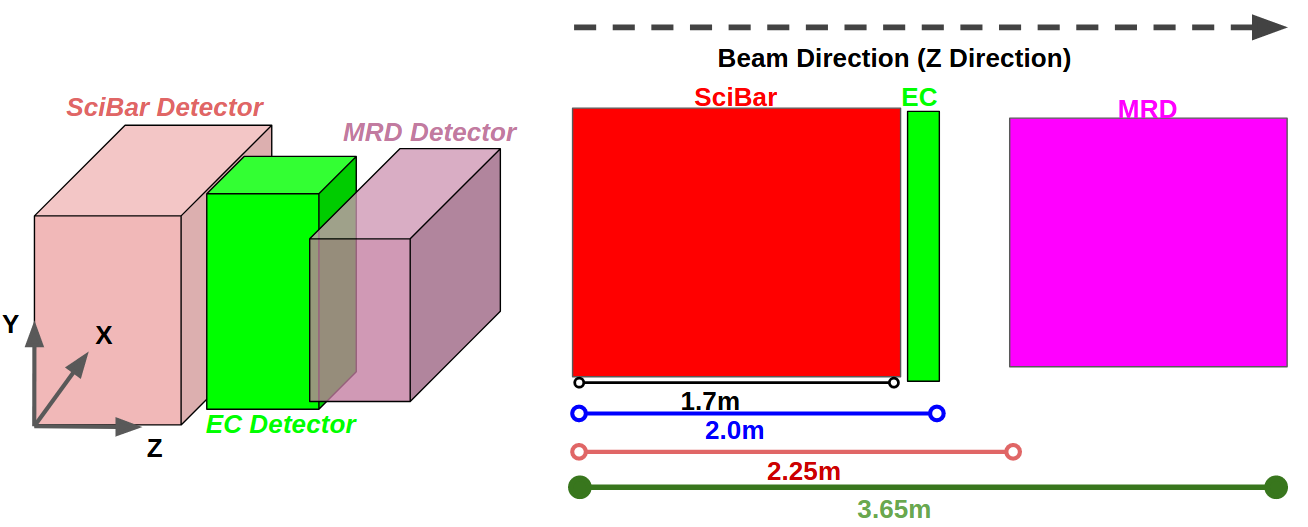
\includegraphics[width=0.75\textwidth]{EventClassifications/SciBooNEDetector.png}
\caption{Representation of the SciBooNE detector and the coordinate frame used in this study}
\label{fig:SciBooNEDetector}
\end{figure}

%----------------------------------------------------------------------|
\subsubsection{The Scintillator Bar Tracker (SciBar)}
\label{subsub:SciBar}
%----------------------------------------------------------------------|
The Scintillator Bar Tracker (SciBar) sub-detector is a scintillator detector which was used to identify neutrino interactions within SciBooNE. The dimensions of the SciBar detector used in this simulation are $0 < x < 3.0$ m, $0 < y < 3.0$ m, and $0 < z < 1.7$ m. This simulation models the scintillator materials as having a constant energy deposition per unit length ($dE/dx$) for both muons and pions of $2.04$ MeV/cm based on previous SciBooNE analyses and on mean values for typical particle momentum listed in the particle data group (PDG).

%----------------------------------------------------------------------|
\subsubsection{The Muon Range Detector (MRD)}
\label{subsub:MRD}
%----------------------------------------------------------------------|
The Muon Range Detector (MRD), depicted in Figure \ref*{fig:mrddetector}, is located $0.55$ $m$ downstream of SciBar in the z-direction, and is a composition of two sets of thirteen alternating slabs of steel-scintillator layers, where the scintillator layers alternate between being horizontally oriented or vertically oriented, in the $xy$-plane. The steel layers have a z-direction thickness of $5.08$ $cm$ and the scintillator layers have a z-direction thickness of $0.6$ $cm$. Combining all the layers of the different alternating materials results in 26 scintillator layers that "sandwich" twenty five steel layers in-between and gives a total z-direction dimension of being $1.37 m$. The xy-plane is modeled as a square again (as was the case with SciBar, too) with dimensions in the x-direction and the y-direction of $2.6$ $m$. The energy deposition per unit length ($dE/dx$) of a muon penetrating the scintillator layers is assumed to be a constant $2.04$ MeV/cm while the energy deposition for the muon in the steel layers is assumed to be a greater value of $11.43$ $MeV/cm$. Both values are typical for muons at the energy range produced in SciBooNE and taken from the PDG.

\begin{figure}[H]
\centering
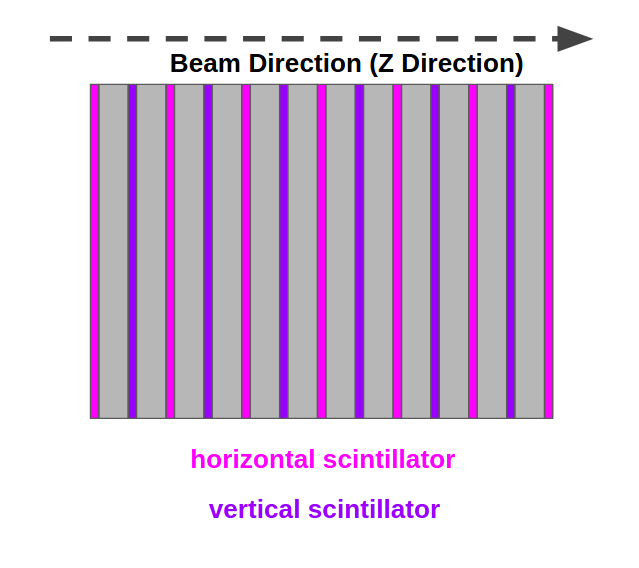
\includegraphics[width=0.75\textwidth]{EventClassifications/mrd.png}
\caption{Depiction of the Muon Range Detector (MRD) which consists of alternating layers of horizontal scintillator (shown in pink) steel slabs (shown in grey) and vertical scintillator (shown in purple)}
\label{fig:mrddetector}
\end{figure}



%=======================================================================
\section{Event Selection}
\label{sec:eventselection}
%=======================================================================
Two main samples are used in this study to generate the acceptance tables. The first is a charged-current inclusive (CC-Inclusive) sample which requires a muon was created in the neutrino interaction and this muon intersects the MRD. This sample is described in Section \ref*{sub:CCInclusive} and is used to validate the building of the acceptance model by comparing it to previous SciBooNE analyses. The second sample is the charged-current coherent pion (CC-Coh $\pi^{+/-}$) sample which requires a muon and charged pion are created in the neutrino interaction exclusively (e.g. no other final state particles in the event). This sample is described in Section \ref*{sub:CCCohPion}.

Both of these samples are selected using NEUT MC-truth flags which ensure we are treating pure samples which are classified by the neutrino generator as belonging to the appropriate sample. Whether or not the event identified by our selection makes it into the final sample used in the acceptance study depends on the behavior of the muon with respect to the MRD. A muon which enters the MRD from a neutrino interaction will either come to stop in the MRD, exit out the back of the MRD (assuming the muon's momentum is great enough), or exit out the side of the MRD. In the subsections below, these classifications are explained further.

%----------------------------------------------------------------------|
\subsection{Muon Stops within the MRD (``Stopped'')}
\label{sub:stoppedMRD}
%----------------------------------------------------------------------|
The requirement to classify a neutrino interaction as a ``stopped'' event requires the muon from the interaction to have reached the MRD, penetrated at least three layers of steel (giving activity in four layers of scintillator), and to then have deposited all of its remaining energy prior to reaching a boundary of the MRD. An illustration of a CC-Coh $\pi$ event that would be classified as ``stopped'' is shown in Figure \ref*{fig:stoppedEvent}.

\begin{figure}[H]
\centering
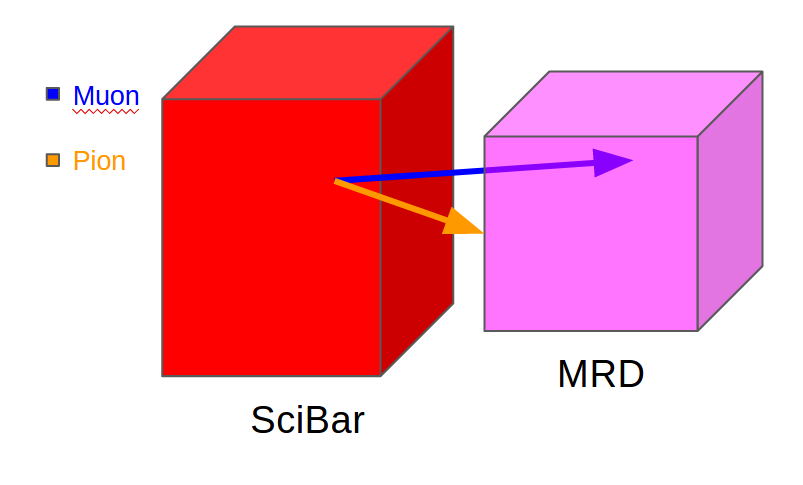
\includegraphics[width=0.6\textwidth]{EventClassifications/Stopped.png}
\caption{Depiction of an event that was classified as ``stopped''.}
\label{fig:stoppedEvent}
\end{figure}

These events allow for complete reconstruction of the muon's momentum based on the number of layers which the muon penetrated and the muon's incident angle.

%----------------------------------------------------------------------|
\subsection{Muon exits out the back of the MRD (``Out-the-back'')}
\label{sub:outback}
%----------------------------------------------------------------------|
The classification of a neutrino interaction as ``out-the-back'' requires the muon from the interaction to have reached the MRD, and to have had sufficient energy such that the muon exited out the back face of the MRD without stopping. An illustration of such an event is given in Figure \ref*{fig:NotStoppedEvent}. 

\begin{figure}[H]
\centering
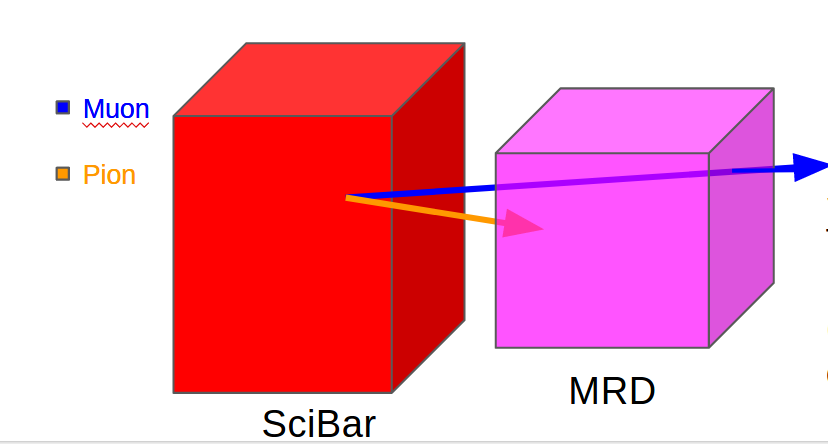
\includegraphics[width=0.6\textwidth]{EventClassifications/NotStopped.png}
\caption{Depiction of an event that was classified as ``out-the-back''.}
\label{fig:NotStoppedEvent}
\end{figure}

The exact momentum of muons which pass completely through the MRD could not be made in reconstruction, so these events were classified as having the minimum energy required to penetrate all the steel and scintillator layers of the MRD.

%----------------------------------------------------------------------|
\subsection{Muon exits out the side of the MRD (``Out-the-side'')}
\label{sub:outside}
%----------------------------------------------------------------------|
The classification of a neutrino interaction as ``out-the-side'' requires that the muon from the interaction reached the MRD, penetrated at least three layers of steel, and then to have exited out the side of the active volume of the MRD (excluding the very back face) without stopping. Events which are classified as ``out-the-side'' are excluded from this study because no accurate reconstruction of the muon's momentum can be made when the muon exits out the side of the MRD. An illustration of such an excluded event which exits out the side of the MRD is given in Figure \ref*{fig:OutTheSideEvent}.


\begin{figure}[H]
\centering
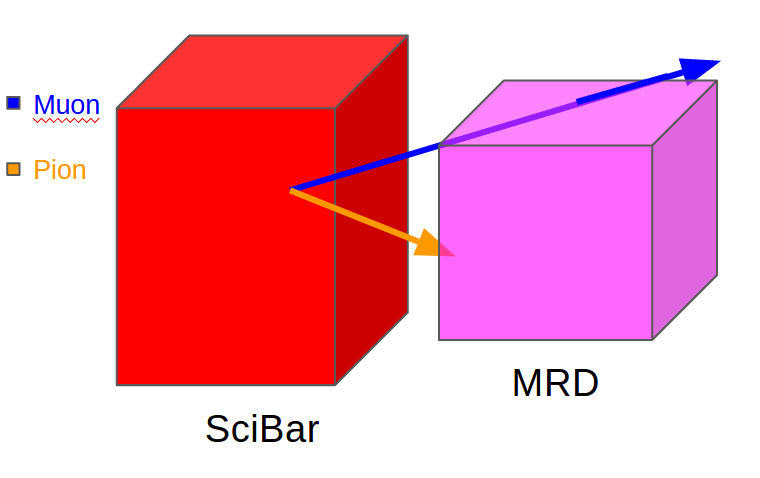
\includegraphics[width=0.6\textwidth]{EventClassifications/OutSide.png}
\caption{Depiction of an event that was classified as ``out-the-side''.}
\label{fig:OutTheSideEvent}
\end{figure}




%=======================================================================
\section{Results}
\label{sec:Results}
%=======================================================================
The results of this acceptance study can be broken down into two different classification schemes of events. Those that met the conditions to qualify as CC-Inclusive events, and those that met the conditions of classification as CC-Coh $\pi$ events. The former is used to validate the acceptance modeling and detector simulation in order to reasonably reproduce previously published CC-Inclusive studies from SciBooNE, while the latter is used for the re-analysis.

%---------------------------------------------------------------------|
\subsection{Charged-Current Inclusive Events}
\label{sub:CCInclusive}
%---------------------------------------------------------------------|

Here we define the CC-Inclusive sample which we use to validate our acceptance model against previously performed simulation studies from SciBooNE.

%---------------------------------------------------------------------|
\subsubsection{$\nu$-mode Charged-Current Inclusive Events}
\label{subsub:NuModeCCInclusive}
%---------------------------------------------------------------------|
Table \ref*{tab:NuCCIncEventReduction} goes through the event selection criteria for selecting a sample of CC-Inclusive events from the $\nu$-mode MC.

\begin{center}
\begin{table}[htb]
	\begin{center}
	\resizebox{0.99\textwidth}{!}{%
	\begin{tabular}{|c|c|c|c|}
	\multicolumn{4}{c}{\textbf{$\nu$-mode CC-Inclusive Event Reduction}} \\
	\hline \hline
	 Events Selection & NEUT v5.3.6 Rein-Sehgal & NEUT v5.3.6 Berger-Sehgal & NEUT v5.0.1 Rein-Sehgal\\
	\hline
	 Total Sample & 1,000,000 & 1,000,000 & 100,000 \\
	\hline
	CC-Inclusive Interaction & 725,730 & 727,278 & 69,363 \\
	($\mu$ + n-other particles in SciBar) & & & \\
	\hline
	Muon enters the MRD & 263,698 & 262,608 & 24,250 \\
	\hline
	Muon enters the MRD and & 231,089 & 230,054 & 21,001 \\
	penetrates $\geq$ 3 layers of steel & & & \\
	\hline
	``Stopped''-Events & 177,406 & 175,799 & 16,062 \\
	``Out-the-back''-Events & 15,389 & 15,952 & 1,421 \\
	``Out-the-side''-Events & 38,294 & 38,303 & 3,518 \\
	\hline
	\hline
	\textbf{Good CC-Inclusive Events} & \textbf{192,795} & \textbf{191,751} & \textbf{17,483} \\
	\hline
	\hline
	\end{tabular}}
	\caption{Event reduction table for a sample of $\nu$-mode CC-Inclusive events simulated in the SciBooNE geometry.}
	\label{tab:NuCCIncEventReduction}
	\end{center}
\end{table}
\end{center}

The first quantity that is calculated for the different events is the momentum of both the muon and the pion, which are both found from the equations:

\begin{equation}
|\vec{p}_\mu| = \sqrt{P_{\mu_x}^2 + P_{\mu_y}^2 + P_{\mu_z}^2}
\end{equation}

\begin{equation}
|\vec{p}_\pi| = \sqrt{P_{\pi_x}^2 + P_{\pi_y}^2 + P_{\pi_z}^2}
\end{equation}

\noindent
where $|\vec{p}_\mu|$ represents the magnitude of the momentum for the corresponding particle, and $P_{\mu_a}$ (where $a$ can be $x$, $y$, $z$, or $E$) represents the component of the four momentum for the corresponding particle. The momentum is reported in units of $MeV/c$.

The next quantity calculated is the angle from the beam-direction for both the muon and the pion, which are labeled as either $\theta_\mu$, or $\theta_\pi$, respectively. The angle from the beam-direction is the same as the angle from the z-direction, and this angle is known as the azimuthal angle in spherical coordinates. The calculation of the azimuthal angle is slightly more involved than the simple calculation used for finding the momentum magnitudes of the two particles, and is calculated using the equations:

\begin{equation}
\theta_\mu = tan^{-1}\Bigg(\frac{\sqrt{P_{\mu_x}^2 + P_{\mu_y}^2}}{P_{\mu_z}}\Bigg)
\end{equation}

\begin{equation}
\theta_\pi = tan^{-1}\Bigg(\frac{\sqrt{P_{\pi_x}^2 + P_{\pi_y}^2}}{P_{\pi_z}}\Bigg)
\end{equation}

\noindent
The angles are reported in units of $\degree$, and should run from $0\degree$ to $180\degree$.

\begin{figure}[H]
\centering
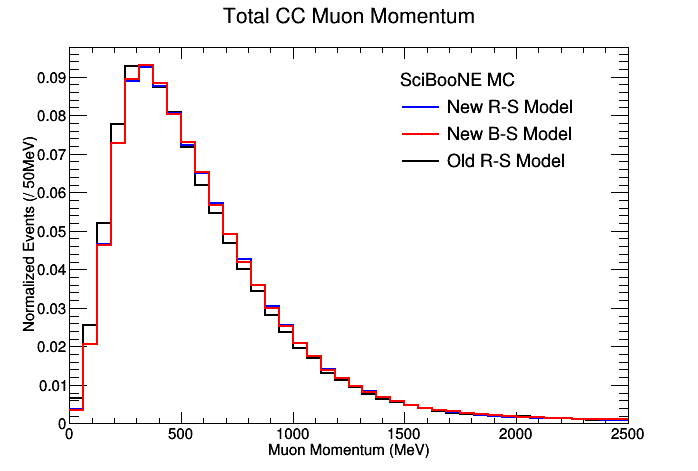
\includegraphics[width=0.4\textwidth]{CCInclusivePlots/NMCCInclusiveTotalMomentum.png}
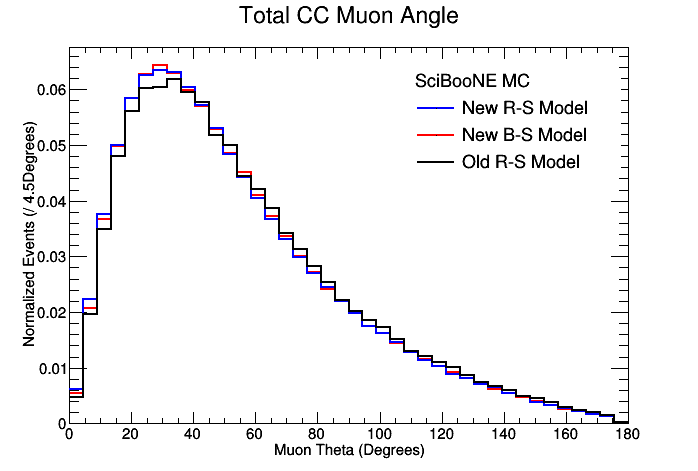
\includegraphics[width=0.4\textwidth]{CCInclusivePlots/NMCCInclusiveTotalAngle.png}
\caption{Muon Momentum (left) and Muon Angle (right) for $\nu$-mode CC-Inclusive interactions for all three models included in this study. These samples kinematics are, unsurprisingly, very similar for the sample of CC-Inclusive.}
\label{fig:NuModeCCInclusiveMomAndAng}
\end{figure}

Figure \ref*{fig:NuModeCCInclusiveMomAndAng} shows the momentum and angular ($\theta_{\mu}$) distribution for the sample of $\nu$-mode CC-Inclusive events passing all of our requirements for all three models considered in this study (NEUT v5.3.6 Rein-Sehgal, NEUT v5.3.6 Berger-Sehgal, NEUT v5.0.1 Rein-Sehgal). The distributions have been normalized to the same area and show no strong differences between them. 

\begin{figure}[H]
\centering
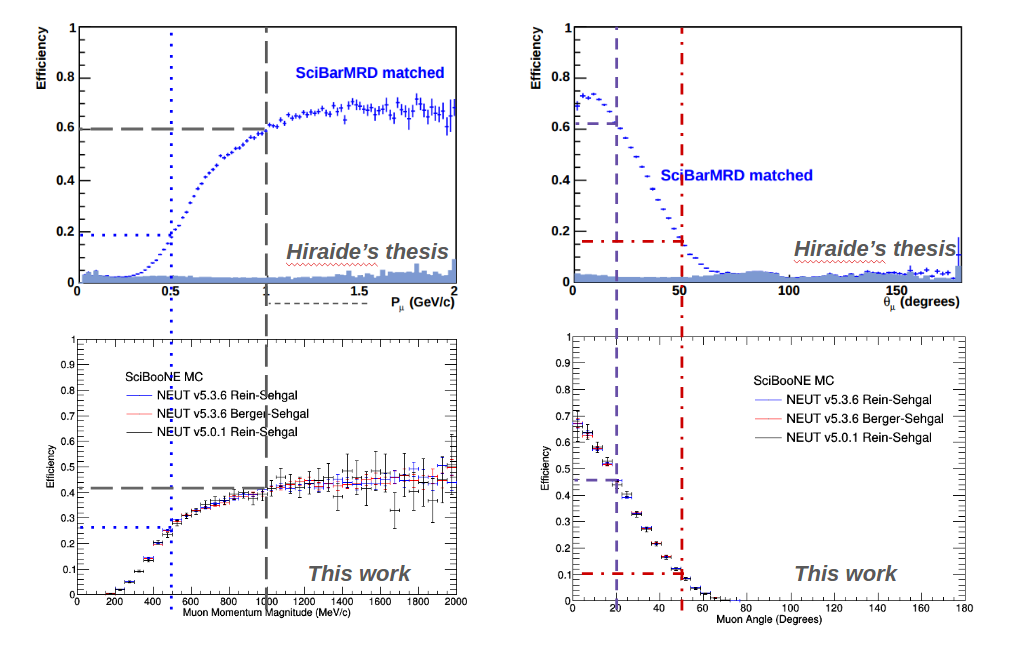
\includegraphics[width=0.8\textwidth]{CCInclusivePlots/CC1DIncEff.png}
\caption{One-dimensional efficiency plots for the $\nu$-mode CC-Inclusive sample.}
\label{fig:OneDEfficiency}
\end{figure}

Figure \ref*{fig:OneDEfficiency} represents the one-dimensional efficiency for selecting $\nu$-mode CC-Inclusive events for this study using all three different models compared to results derived from Hiraide's thesis \footnote{Hiraide's thesis can be found here: \href{http://www-he.scphys.kyoto-u.ac.jp/theses/doctor/hiraide_dt.pdf}{http://www-he.scphys.kyoto-u.ac.jp/theses/doctor/hiraide\textunderscore{}dt.pdf}} using the full SciBooNE Monte Carlo simulation. A few reference points are illustrated using dashed lines to guide the readers eye. A few perecent difference is seen, but overall agreement between the two simulations hold.

Below are the two dimensional efficiency plots for the CC-Inclusive events in $\nu$ mode. The tables that correspond to the plots can be found in the Efficiency Tables section of the Appendix under the Charged-Current Inclusive Sample Efficiency Tables subsection.

\begin{figure}[H]
\centering
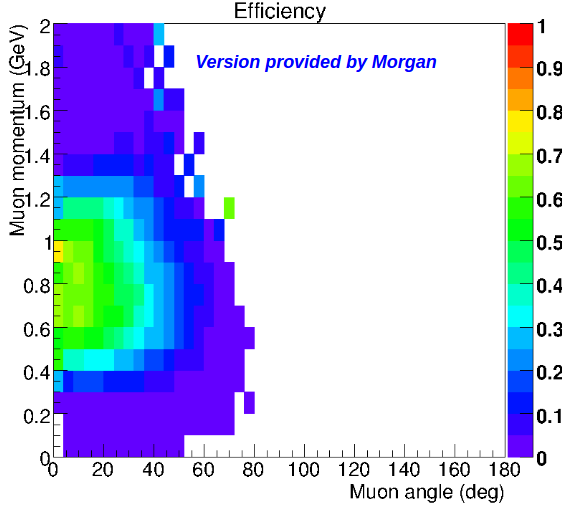
\includegraphics[width=0.3\textwidth]{CCInclusivePlots/MorgansCCInclusiveSample.png}
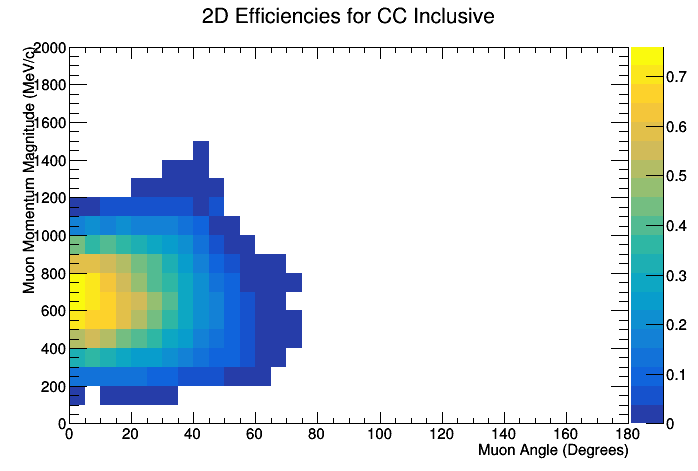
\includegraphics[width=0.4\textwidth]{CCInclusivePlots/2DEffCompareNMRS.png}
\caption{Reference plot provided by Morgan (left), and the two-dimensional efficiency plot for CC-Inclusive events in $\nu$-mode NEUT v5.3.6 Rein-Sehgal MC (right).}
\label{fig:TwoDEfficiencyRS}
\end{figure}

Figure \ref*{fig:TwoDEfficiencyRS} shows the two-dimensional efficiency for selecting $\nu$-mode CC-Inclusive events in the NEUT v5.3.6 Rein-Sehgal MC. The left hand side is a reference plot provided by Morgan and the right hand side is for the NEUT v5.3.6 Rein-Sehgal MC used in this study. Table \ref*{tab:app:CCIncNMRS} is the efficiency table that corresponds to the two-dimensional efficiency plot on the right of Figure \ref*{fig:TwoDEfficiencyRS}.

\begin{figure}[H]
\centering
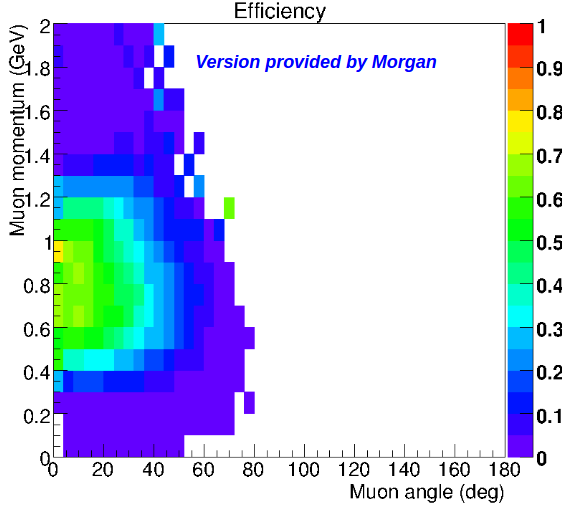
\includegraphics[width=0.3\textwidth]{CCInclusivePlots/MorgansCCInclusiveSample.png}
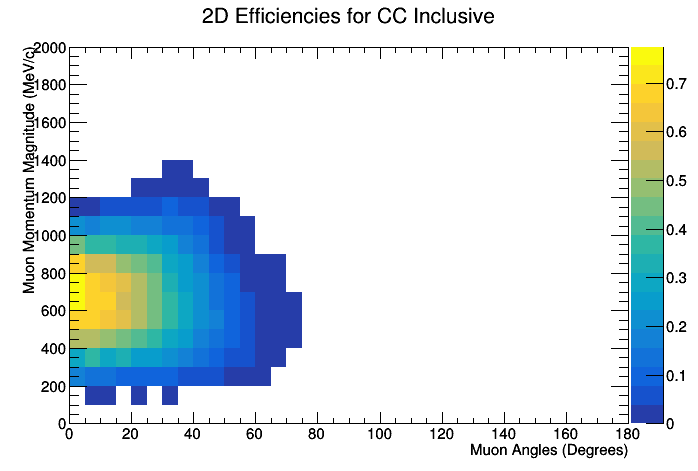
\includegraphics[width=0.4\textwidth]{CCInclusivePlots/2DEffCompareNMBS.png}
\caption{Reference plot provided by Morgan (left), and the two-dimensional efficiency plot for CC-Inclusive events in $\nu$-mode NEUT v5.3.6 Berger-Sehgal MC (right).}
\label{fig:TwoDEfficiencyBS}
\end{figure}

Figure \ref*{fig:TwoDEfficiencyBS} shows the two-dimensional efficiency for selecting $\nu$-mode CC-Inclusive events in the NEUT v5.3.6 Berger-Sehgal MC. The left hand side is a reference plot provided by Morgan and the right hand side is for the NEUT v5.3.6 Berger-Sehgal MC used in this study. Table \ref*{tab:app:CCIncNMBS} is the efficiency table that corresponds to the two-dimensional efficiency plot on the right of Figure \ref*{fig:TwoDEfficiencyBS}.

\begin{figure}[H]
\centering
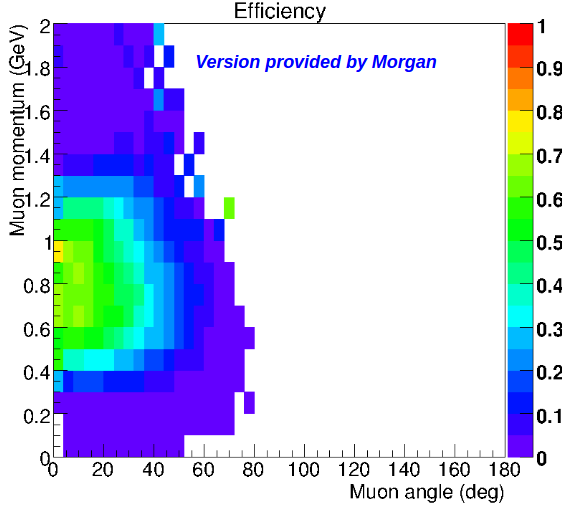
\includegraphics[width=0.3\textwidth]{CCInclusivePlots/MorgansCCInclusiveSample.png}
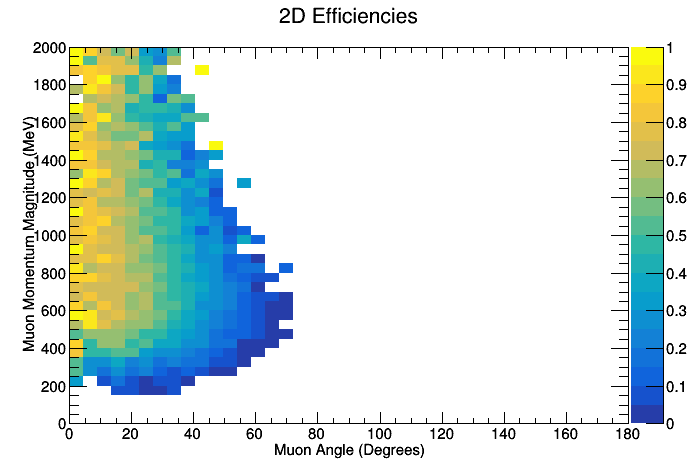
\includegraphics[width=0.4\textwidth]{CCInclusivePlots/2DEffCompareNMORS.png}
\caption{Reference plot provided by Morgan (left), and the two-dimensional efficiency plot for CC-Inclusive events in $\nu$-mode NEUT v5.0.1 Rein-Sehgal MC (right).}
\label{fig:TwoDEfficiencyORS}
\end{figure}

Figure \ref*{fig:TwoDEfficiencyORS} shows the two-dimensional efficiency for selecting $\nu$-mode CC-Inclusive events in the NEUT v5.0.1 Rein-Sehgal MC. The left hand side is a reference plot provided by Morgan and the right hand side is for the NEUT v5.0.1 Rein-Sehgal MC used in this study. Table \ref*{tab:app:CCIncNMORS} is the efficiency table that corresponds to the two-dimensional efficiency plot on the right of Figure \ref*{fig:TwoDEfficiencyORS}.

%---------------------------------------------------------------------|
\subsubsection{$\bar{\nu}$-mode Charged-Current Inclusive Events}
\label{subsub:antiNuModeCCInclusive}
%---------------------------------------------------------------------|

Similar to before, Table \ref*{tab:AntiNuCCIncEventReduction} goes through the event selection criteria for selecting a sample of CC-Inclusive events from the $\bar{\nu}$-mode MC.


\begin{center}
\begin{table}[htb]
	\begin{center}
	\resizebox{0.99\textwidth}{!}{%
	\begin{tabular}{|c|c|c|}
	\multicolumn{3}{c}{\textbf{$\bar{\nu}$-mode CC-Inclusive Event Reduction}} \\
	\hline \hline
	 Events Selection & NEUT v5.3.6 Rein-Sehgal & NEUT v5.3.6 Berger-Sehgal \\
	\hline
	 Total Sample & 1,000,000 & 1,000,000 \\
	\hline
	CC-Inclusive Interaction & 699,239 & 704,327 \\
	($\mu$ + n-other particles in SciBar) & & \\
	\hline
	Muon enters the MRD & 380,362 & 380,869 \\
	\hline
	Muon enters the MRD and & 336,373 & 337,979 \\
	penetrates $\geq$ 3 layers of steel & & \\
	\hline
	``Stopped''-Events & 288,289 & 288,206 \\
	``Out-the-back''-Events & 7,608 & 7,857 \\
	``Out-the-side''-Events & 40,476 & 41,916 \\
	\hline
	\hline
	\textbf{Good CC-Inclusive Events} & \textbf{295,897} & \textbf{296,063} \\
	\hline
	\hline
	\end{tabular}}
	\caption{Event reduction table for a sample of $\bar{\nu}$-mode CC-Inclusive events simulated in the SciBooNE geometry.} 
	\label{tab:AntiNuCCIncEventReduction}
	\end{center}
\end{table}
\end{center} 

\begin{figure}[H]
\centering
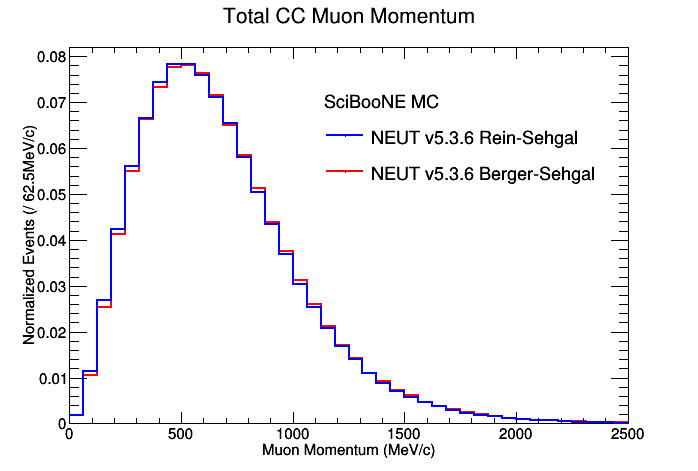
\includegraphics[width=0.4\textwidth]{CCInclusivePlots/ANMCCInclusiveTotalMomentum.png}
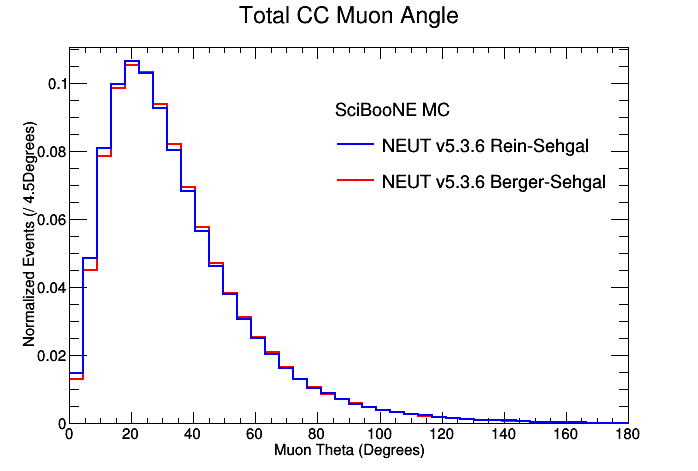
\includegraphics[width=0.4\textwidth]{CCInclusivePlots/ANMCCInclusiveTotalAngle.png}
\caption{Muon momentum (left) and muon angle (right) for $\bar{\nu}$-mode CC-Inclusive interactions for both models included in this study. These samples' kinematics are, unsurprisingly, very similar for the sample of CC-Inclusive.}
\label{fig:AntiNuCCInclusiveMomAndAngle}
\end{figure}

Figure \ref*{fig:AntiNuCCInclusiveMomAndAngle} shows the momentum and angular distribution for the sample of $\bar{\nu}$-mode CC-Inclusive events passing all our requirements for both models considered in this study (NEUT v5.3.6 Rein-Sehgal, and NEUT v5.3.6 Berger-Sehgal). The distributions have been normalized to the same area and show no strong differences between them.

\begin{figure}[H]
\centering
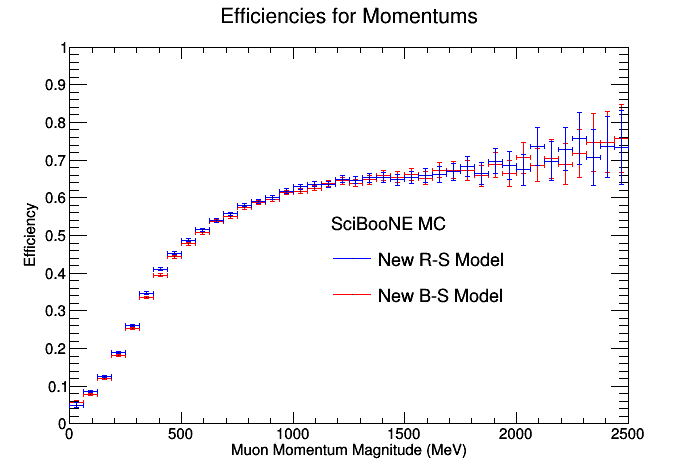
\includegraphics[width=0.4\textwidth]{ANMCombinedPlotsImages/16-ANMCombinedPlots.png}
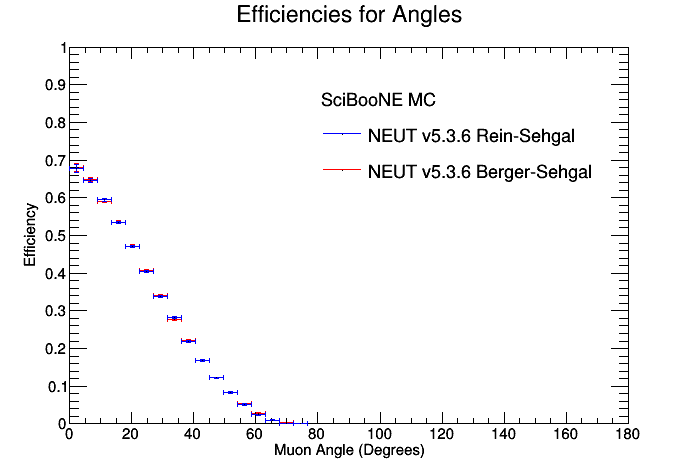
\includegraphics[width=0.4\textwidth]{ANMCombinedPlotsImages/15-ANMCombinedPlots.png}
\caption{One-dimensional efficiency plots for the CC-Inclusive events in the $\bar{\nu}$-mode MCs. Muon momentum is on the right and the muon angle is on the left.}
\label{fig:OneDEfficiencyAntiNu}
\end{figure}

Figure \ref*{fig:OneDEfficiencyAntiNu} represents the one-dimensional efficiency for selecting $\bar{\nu}$-mode CC-Inclusive events for this study. No similar reference sample exists to be compared directly against, however we note that the shape and magnitude of the acceptance is nearly unchanged between $\bar{\nu}$ and $\nu$-mode samples (as expected).

Below are the two dimensional efficiency plots for the CC-Inclusive events in $\bar{\nu}$ mode. The tables that correspond to the plots can be found in the Efficiency Tables section of the Appendix under the Charged-Current Inclusive Sample Efficiency Tables subsection.

\begin{figure}[H]
\centering
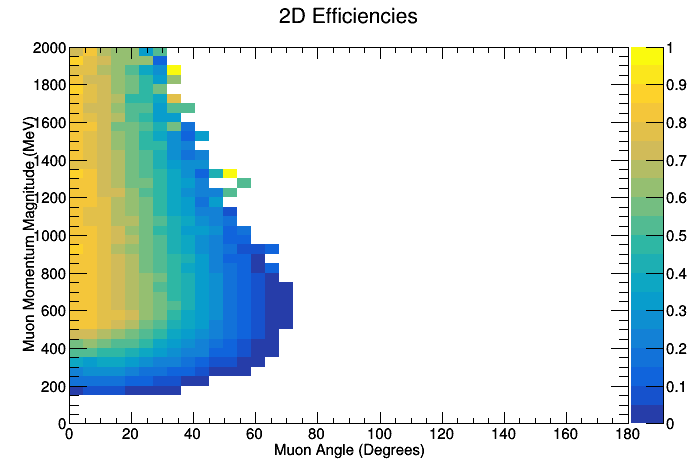
\includegraphics[width=0.6\textwidth]{CCInclusivePlots/2DEffCompareANMRS.png}
\caption{Two-dimensional efficiency plot for the CC-Inclusive events of the $\bar{\nu}$-mode NEUT v5.3.6 Rein-Sehgal MC.}
\label{fig:ANMTwoDEfficiencyRS}
\end{figure}

Figure \ref*{fig:ANMTwoDEfficiencyRS} shows the two-dimensional efficiency for selecting $\bar{\nu}$-mode CC-Inclusive events in NEUT v5.3.6 Rein-Sehgal MC. Table \ref*{tab:app:CCIncANMRS} is the efficiency table that corresponds to the two-dimensional efficiency plot in Figure \ref*{fig:ANMTwoDEfficiencyRS}.

\begin{figure}[H]
\centering
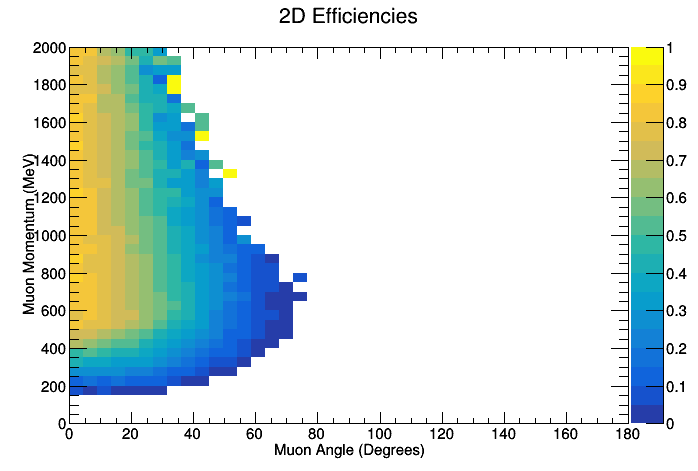
\includegraphics[width=0.6\textwidth]{CCInclusivePlots/2DEffCompareANMBS.png}
\caption{Two-dimensional efficiency plot for the CC-Inclusive events of the $\bar{\nu}$-mode NEUT v5.3.6 Berger-Sehgal MC.}
\label{fig:ANMTwoDEfficiencyBS}
\end{figure}

Figure \ref*{fig:ANMTwoDEfficiencyBS} shows the two-dimensional efficiency for selecting $\bar{\nu}$-mode CC-Inclusive events in NEUT v5.3.6 Berger-Sehgal MC. Table \ref*{tab:app:CCIncANMBS} is the efficiency table that corresponds to the two-dimensional efficiency plot in Figure \ref*{fig:ANMTwoDEfficiencyBS}.


%---------------------------------------------------------------------|
\subsection{Charged-Current Coherent Pion Production Events}
\label{sub:CCCohPion}
%---------------------------------------------------------------------|

Here we define the CC-Coh $\pi$ sample which will be used in the re-analysis. The momentum and angle equations that were used above for the CC-Inclusive events were also used for the CC-Coh $\pi$ events.

%---------------------------------------------------------------------|
\subsubsection{$\nu$-mode Charged-Current Coherent Pion Events}
\label{subsub:NuModeCCCohPion}
%---------------------------------------------------------------------|

Table \ref*{tab:NuCCCoherentEventReduction} goes through the event selection criteria for selecting a sample of CC-Coh $\pi$ events from the $\nu$-mode MC.

\begin{center}
\begin{table}[htb]
	\begin{center}
	\resizebox{0.99\textwidth}{!}{%
	\begin{tabular}{|c|c|c|c|}
	\multicolumn{4}{c}{\textbf{$\nu$-mode CC-Coherent Pion Event Reduction}} \\
	\hline \hline
	 Events Selection & NEUT v5.3.6 Rein-Sehgal & NEUT v5.3.6 Berger-Sehgal & NEUT v5.0.1 Rein-Sehgal\\
	\hline
	Total Sample & 1,000,000 & 1,000,000 & 100,000 \\
	\hline
	CC-Coherent Pion Interaction & 12,186 & 2,576 & 1,320 \\
	($\mu$ + $\pi$ + $\varnothing$ in SciBar) & & & \\
	\hline
	Both muon and pion are  & 8,535 & 1,845 & 884 \\
	forward going &  &  &  \\
	\hline
	Muon enters the MRD and & 7,407 & 1,592 & 767 \\
	penetrates $\geq$ 3 layers of steel & & & \\
	\hline
	``Stopped''-Events & 6,448 & 1,350 & 669 \\
	``Out-the-back''-Events & 530 & 150 & 56 \\
	``Out-the-side''-Events & 429 & 92 & 42 \\
	\hline
	\hline
	\textbf{Good Coherent Pion Events} & \textbf{6,978} & \textbf{1,500} & \textbf{725} \\
	\hline
	\hline
	\end{tabular}}
	\caption{Event reduction table for a sample of $\nu$-mode CC-Coh $\pi$ events simulated in the SciBooNE geometry.}
	\label{tab:NuCCCoherentEventReduction} 
	\end{center}
\end{table}
\end{center}


\begin{figure}[H]
\centering
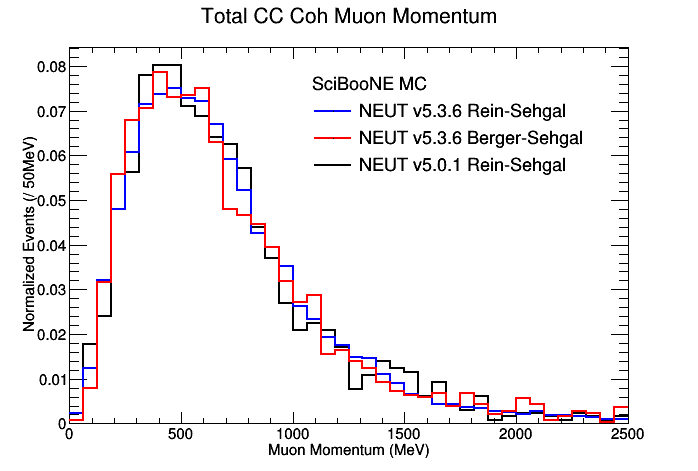
\includegraphics[width=0.4\textwidth]{CCCohPlots/NMCCCohTotalMomentum.png}
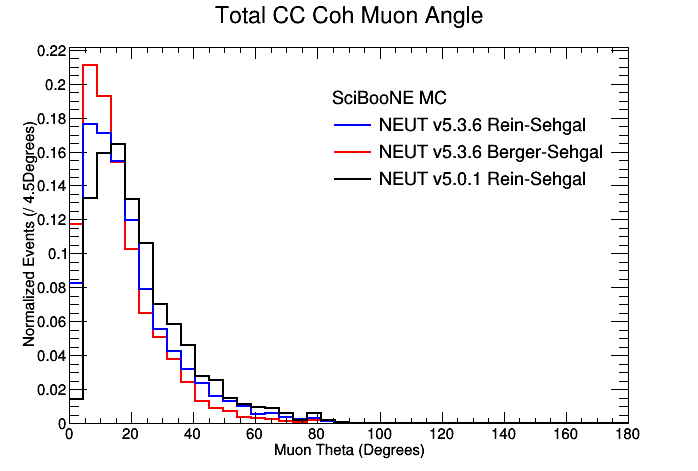
\includegraphics[width=0.4\textwidth]{CCCohPlots/NMCCCohTotalAngle.png}
\caption{Muon momentum for all of the muons of the events that made it to the MRD (left) and muon angle for the muons of the events that made it to the MRD (right) for $\nu$-mode CC-Coh $\pi$ interactions of all three models used in this study. The ``Total'' classification means that all three classifications for the CC-Coh $\pi$ events (``stopped'', ``out-the-side'', and ``out-the-back'') are included.}
\label{fig:NuModeCCCohTotalMomAndAng}
\end{figure}


\begin{figure}[H]
\centering
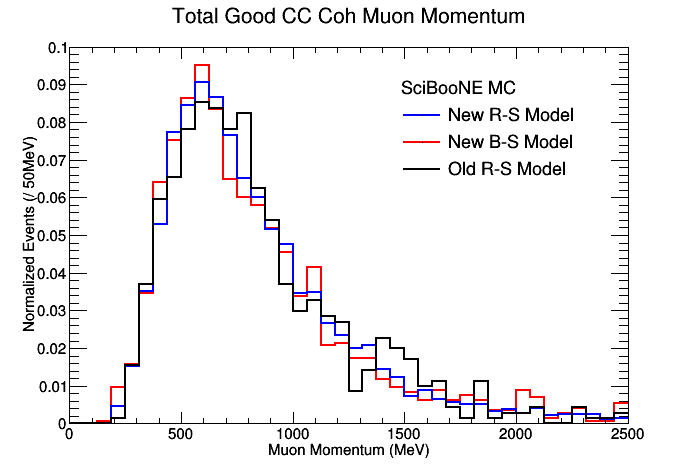
\includegraphics[width=0.4\textwidth]{CCCohPlots/NMCCCohGoodMomentum.png}
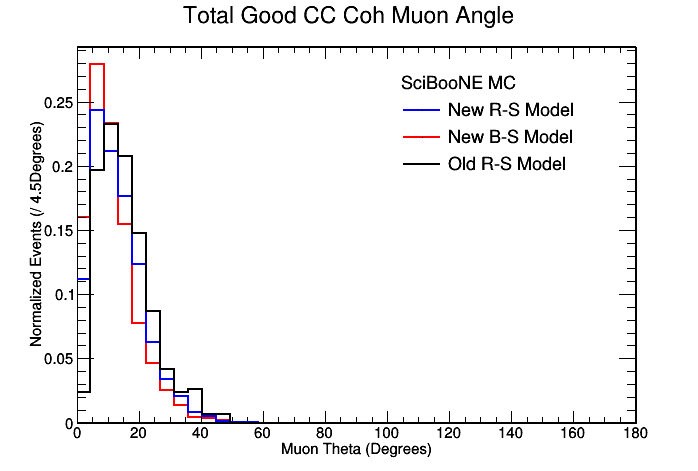
\includegraphics[width=0.4\textwidth]{CCCohPlots/NMCCCohGoodAngle.png}
\caption{Muon momentum of both the ``stopped'' and the ``out-the-back'' samples (left) and muon angle of both the ``stopped'' and the ``out-the-back'' samples (right) for $\nu$-mode CC-Coh $\pi$ interactions of all three models included in this study. The ``Good'' classification means that only the ``stopped'' and the ``out-the-back'' CC-Coh $\pi$ events that the muon penetrated at least four layers of scintillator of the MRD are included for these histograms.}
\label{fig:NuModeCCCohGoodMomAndAng}
\end{figure}


The last two quantities that are calculated are the two different types of four-momentum transfers specific to this interaction, which are $Q^2$ and $|t|$. The $Q^2$ corresponds to the four-momentum transfer from the neutrino and muon to the nucleus and pion, and is calculated using the equation:

\begin{equation}
Q^2 = |(P_{\nu_\mu} - P_\mu)^2|
\end{equation}

\noindent
This equation is in four-momentum notational form. The code follows the equation below in order to compute $Q^2$:

\begin{equation}
Q^2 = |(P_{\nu_{\mu,x}} - P_{\mu_x})^2 + (P_{\nu_{\mu,y}} - P_{\mu_y})^2 + (P_{\nu_{\mu,z}} - P_{\mu_z})^2 + (P_{\nu_{\mu,E}} - P_{\mu_E})^2|
\end{equation}

\noindent
$Q^2$ is reported in units of $(MeV/c)^2$.

The $|t|$ corresponds to the four-momentum transfer from the neutrino, muon, and pion to the nucleus, and is calculated using the equation:

\begin{equation}
|t| = |(Q - P_\pi)^2| = |(P_{\nu_\mu} - P_\mu - P_\pi)^2|
\end{equation}

\noindent
This equation is in four-momentum notational form. The code follows the equation below in order to compute $|t|$:

\begin{equation}
|t| = |(P_{\nu_{\mu,x}} - P_{\mu_x} - P_{\pi_x})^2 + (P_{\nu_{\mu,y}} - P_{\mu_y} - P_{\pi_y})^2 + (P_{\nu_{\mu,z}} - P_{\mu_z} - P_{\pi_z})^2 + (P_{\nu_{\mu,E}} - P_{\mu_E} - P_{\pi_E})^2|
\end{equation}

\noindent
$|t|$ is reported in units of $(MeV/c)^2$.


$\nu$-mode $|t|$ and $Q^2$ plots are below.

\begin{figure}[H]
\centering
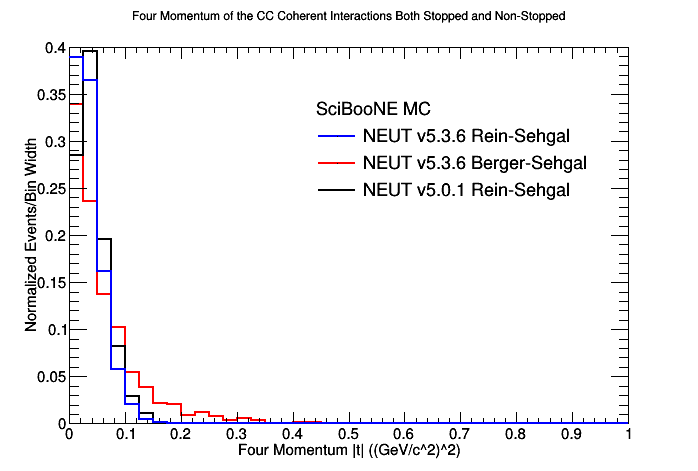
\includegraphics[width=0.4\textwidth]{CCCohPlots/NMCCCohGoodT.png}
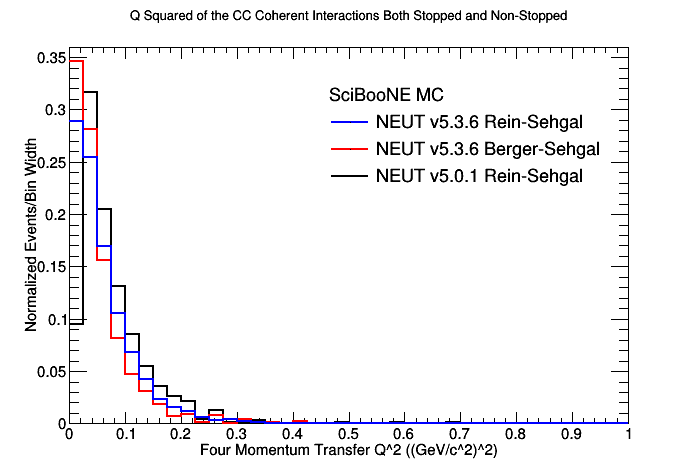
\includegraphics[width=0.4\textwidth]{CCCohPlots/NMCCCohGoodQ2.png}
\caption{The $|t|$ momentum transfer for the ``stopped'' and the ``out-the-back'' events (left) and $Q^2$ momentum transfer for the ``stopped'' and the ``out-the-back'' events (right) for $\nu$-mode CC-Coh $\pi$ interactions for the three models included in this study.} 
\label{fig:NuModeCCCohGoodTAndQ2}
\end{figure}





\begin{figure}[H]
\centering
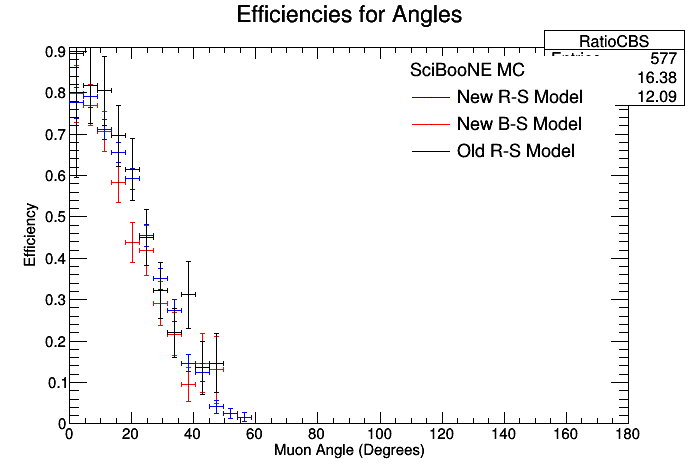
\includegraphics[width=0.4\textwidth]{NMCombinedPlotsImages/24-NMCombinedPlots.png}
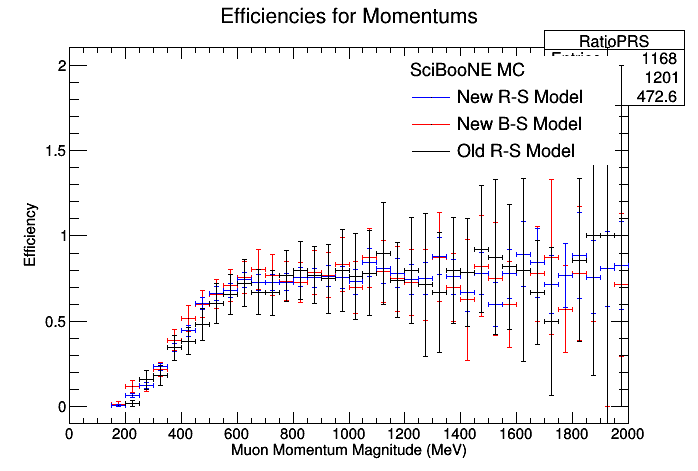
\includegraphics[width=0.4\textwidth]{NMCombinedPlotsImages/25-NMCombinedPlots.png}
\caption{These two plots are the one-dimensional efficiency plots of the muon information. The left plot is the muon angle efficiency plot and the right is the muon momentum efficiency plot for $\nu$-mode.}
\label{fig:MomAngEffNM}
\end{figure}


Below are the two-dimensional efficiency plots for the CC-Coh $\pi$ events in $\nu$-mode for all three models used in this acceptance study (NEUT v5.3.6 Rein-Sehgal, NEUT v5.3.6 Berger-Sehgal, and NEUT v5.0.1 Rein-Sehgal). The tables that correspond to the plots can be found in the Efficiency Tables section of the Appendix within the Charged-Current Coherent Pion Production Efficiency Tables subsection.

\begin{figure}[H]
\centering
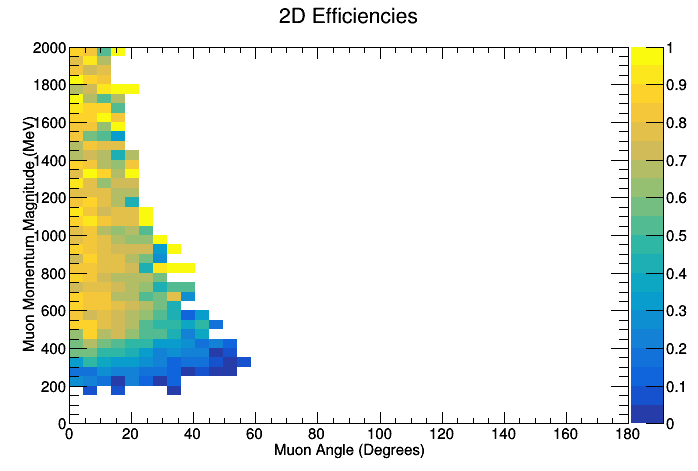
\includegraphics[width=0.6\textwidth]{CCCohPlots/2DEffNMRS.png}
\caption{Two-dimensional efficiency plot for the CC-Coh $\pi$ events of the $\nu$-mode NEUT v5.3.6 Rein-Sehgal MC. Table \ref*{tab:app:CCCohNMRS} is the efficiency table for this two-dimensional efficiency histogram.}
\label{fig:TwoDEfficiencyCCCohNMRS}
\end{figure}

\begin{figure}[H]
\centering
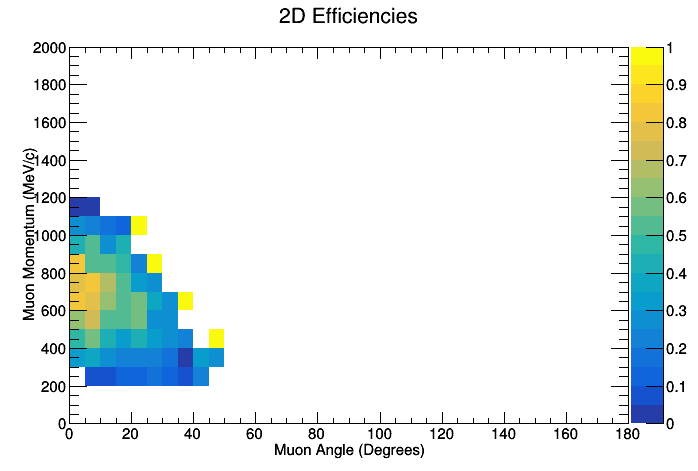
\includegraphics[width=0.6\textwidth]{CCCohPlots/2DEffNMBS.png}
\caption{Two-dimensional efficiency plot for the CC-Coh $\pi$ events of the $\nu$-mode NEUT v5.3.6 Berger-Sehgal MC. Table \ref*{tab:app:CCCohNMBS} is the efficiency table for this two-dimensional efficiency histogram.}
\label{fig:TwoDEfficiencyCCCohNMBS}
\end{figure}

\begin{figure}[H]
\centering
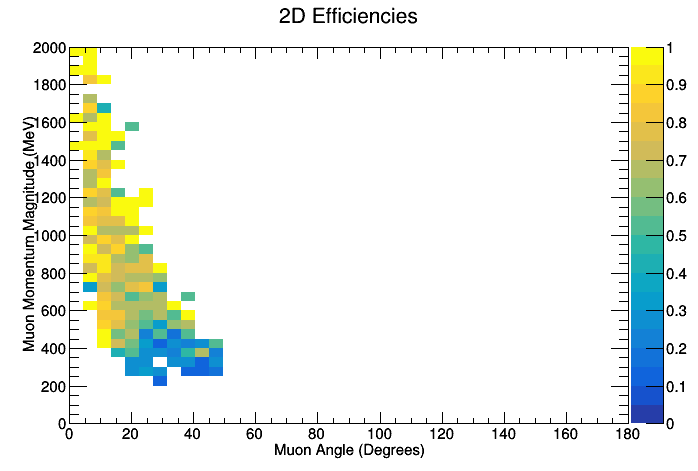
\includegraphics[width=0.6\textwidth]{CCCohPlots/2DEffNMORS.png}
\caption{Two-dimensional efficiency plot for the CC-Coh $\pi$ events of the $\nu$-mode NEUT v5.0.1 Rein-Sehgal MC. Table \ref*{tab:app:CCCohNMORS} is the efficiency table for this two-dimensional efficiency histogram.}
\label{fig:TwoDEfficiencyCCCohNMORS}
\end{figure}

%---------------------------------------------------------------------|
\subsubsection{$\bar{\nu}$-mode Charged-Current Coherent Pion Events}
\label{subsub:AntiNuModeCCCohPion}
%---------------------------------------------------------------------|

Similar to before, Table \ref{tab:AntiNuCCCoherentEventReduction} goes through the event selection criteria for selecting a sample of CC-Coh $\pi$ events from the $\bar{\nu}$-mode MC.

\begin{center}
\begin{table}[htb]
	\begin{center}
	\resizebox{0.99\textwidth}{!}{%
	\begin{tabular}{|c|c|c|}
	\multicolumn{3}{c}{\textbf{$\bar{\nu}$-mode CC-Coherent Pion Event Reduction}} \\
	\hline \hline
	 Events Selection & NEUT v5.3.6 Rein-Sehgal & NEUT v5.3.6 Berger-Sehgal \\
	\hline
	Total Sample & 1,000,000 & 1,000,000 \\
	\hline
	CC-Coherent Pion Interaction & 36,669 & 7,790 \\
	($\mu$ + $\pi$ + $\varnothing$ in SciBar) & & \\
	\hline
	Both muon and pion are  & 24,675 & 5,477 \\
	forward going & & \\
	\hline
	Muon enters the MRD and & 20,445 & 4,517 \\
	penetrates $\geq$ 3 layers of steel & & \\
	\hline
	``Stopped''-Events & 18,935 & 4,203 \\
	``Out-the-back''-Events & 372 & 82 \\
	``Out-the-side''-Events & 1,138 & 232 \\
	\hline
	\hline
	\textbf{Good Coherent Pion Events} & \textbf{19,307} & \textbf{4,285} \\
	\hline
	\hline
	\end{tabular}}
	\caption{Event reduction table for a sample of $\bar{\nu}$-mode CC-Coh $\pi$ events simulated in the SciBooNE geometry.}
	\label{tab:AntiNuCCCoherentEventReduction}
	\end{center}
\end{table}
\end{center}

Below are the plots for CC-Coh $\pi$ events for $\bar{\nu}$-mode. The layout of the rest will be very similar to $\nu$-mode, and the equations used previously for the momentums and angles are the same equations used for the variables of the histograms that follow.

\begin{figure}[H]
\centering
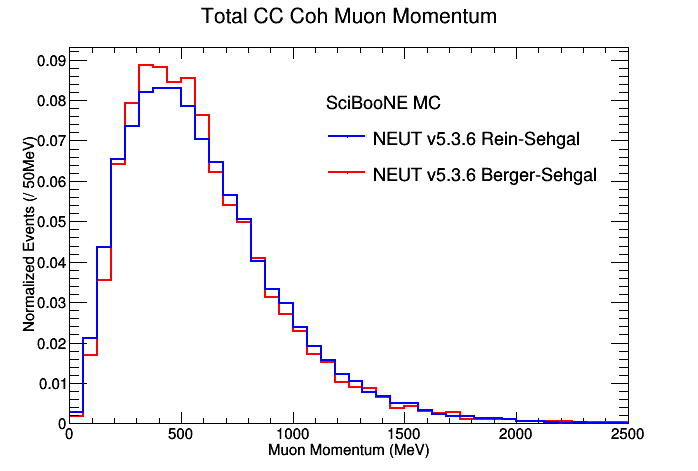
\includegraphics[width=0.4\textwidth]{CCCohPlots/ANMCCCohTotalMomentum.png}
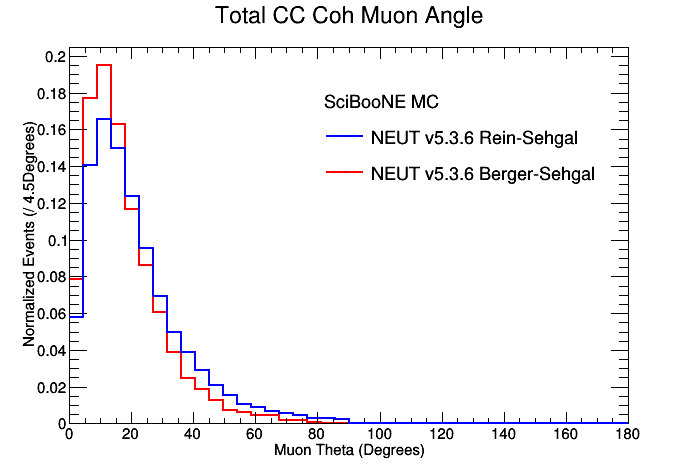
\includegraphics[width=0.4\textwidth]{CCCohPlots/ANMCCCohTotalAngle.png}
\caption{Muon momentum (left) and muon angle (right) for $\bar{\nu}$-mode CC-Coh $\pi$ interactions for both the NEUT v5.3.6 Rein-Sehgal and the NEUT v5.3.6 Berger-Sehgal samples included in this study.}
\label{fig:AntiNuModeCCCohTotalMomAndAng}
\end{figure}

The structure of the plots in Figure \ref*{fig:AntiNuModeCCCohTotalMomAndAng} very closely resemble the same plots in $\nu$-mode above. The rest of the plots in this section have that same characteristic.

\begin{figure}[H]
\centering
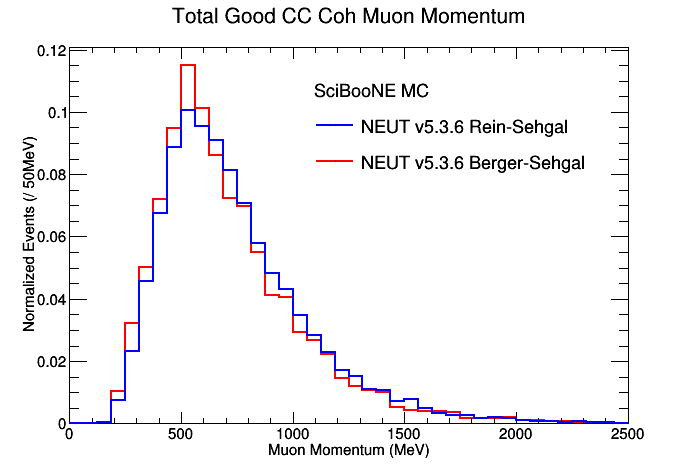
\includegraphics[width=0.4\textwidth]{CCCohPlots/ANMCCCohGoodMomentum.png}
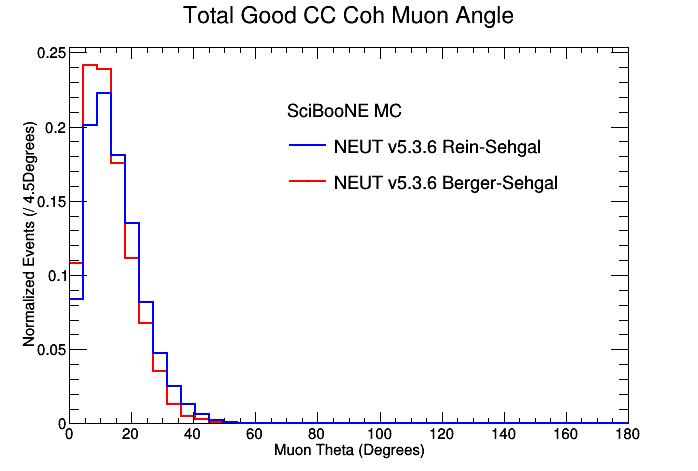
\includegraphics[width=0.4\textwidth]{CCCohPlots/ANMCCCohGoodAngle.png}
\caption{Muon momentum (left) and muon angle (right) for $\bar{\nu}$-mode CC-Coh $\pi$ interactions for both the ``stopped'' and ``out-the-back'' classification of events in both the NEUT v5.3.6 Rein-Sehgal and the NEUT v5.3.6 Berger-Sehgal samples.}
\label{fig:AntiNuModeCCCohGoodMomAndAng}
\end{figure}

$\bar{\nu}$-mode $|t|$ and $Q^2$ plots are below. They also have the same overall shape as the plots for $\nu$-mode above.

\begin{figure}[H]
\centering
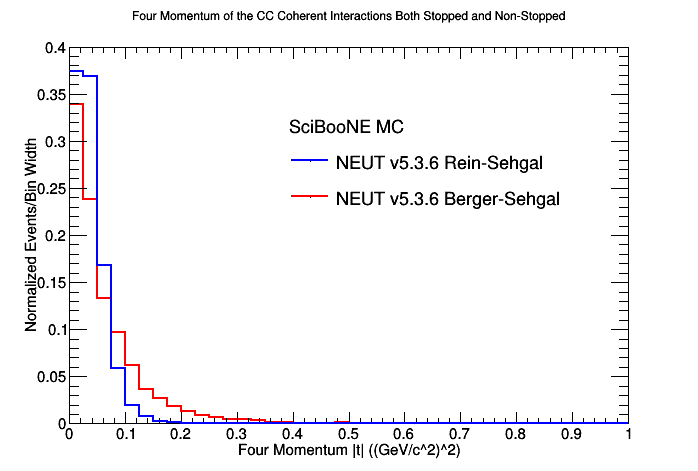
\includegraphics[width=0.4\textwidth]{CCCohPlots/ANMCCCohGoodT.png}
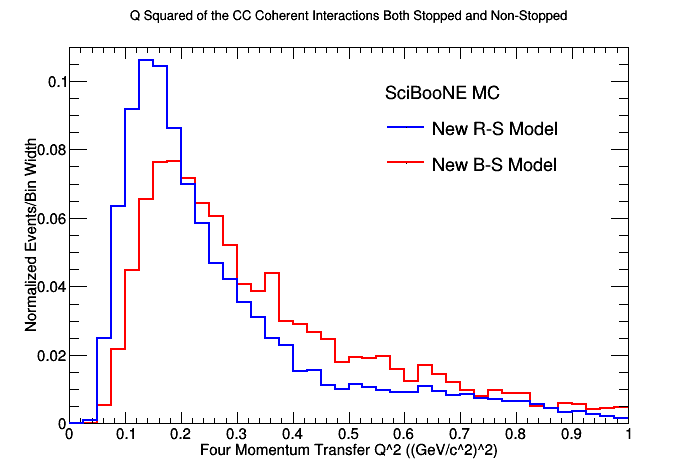
\includegraphics[width=0.4\textwidth]{CCCohPlots/ANMCCCohGoodQ2.png}
\caption{The $|t|$ momentum transfer for the ``stopped'' and the ``out-the-back'' events (left) and $Q^2$ momentum transfer for the ``stopped'' and the ``out-the-back'' events (right) for $\bar{\nu}$-mode CC-Coh $\pi$ interactions for both models included in this study.}
\label{fig:AntiNuModeCCCohGoodTAndQ2}
\end{figure}





\begin{figure}[H]
\centering
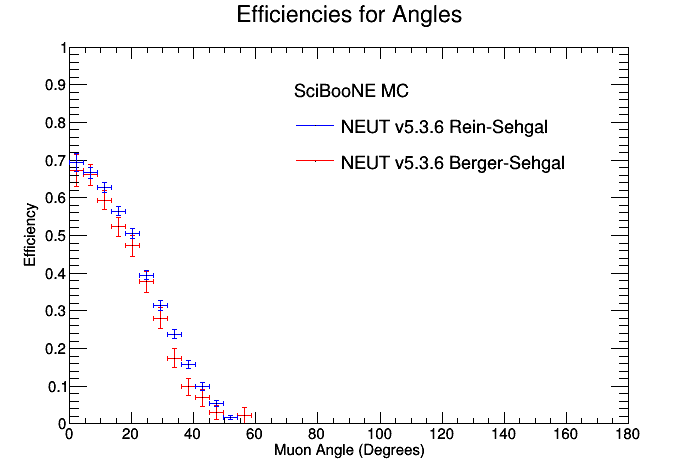
\includegraphics[width=0.4\textwidth]{ANMCombinedPlotsImages/17-ANMCombinedPlots.png}
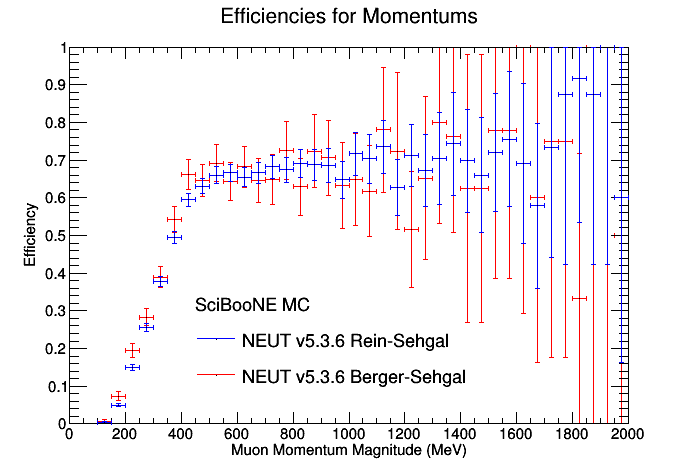
\includegraphics[width=0.4\textwidth]{ANMCombinedPlotsImages/18-ANMCombinedPlots.png}
\caption{These two plots are the one-dimensional efficiency plots of the muon information. The left plot is the muon angle efficiency plot and the right is the muon momentum efficiency plot for $\bar{\nu}$-mode.}
\label{fig:MomAngEffANM}
\end{figure}


Below are the two-dimensional efficiency plots for the CC-Coh $\pi$ events in $\bar{\nu}$-mode. The tables that correspond to the plots can be found in the Efficiency Tables section of the Appendix in the Charged-Current Coherent Pion Production Efficiency Tables subsection.

\begin{figure}[H]
\centering
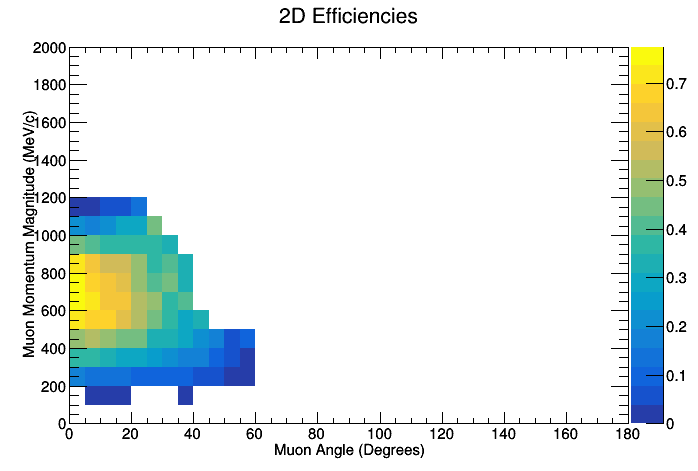
\includegraphics[width=0.6\textwidth]{CCCohPlots/2DEffANMRS.png}
\caption{Two-dimensional efficiency plot for the CC-Coh $\pi$ events of the $\bar{\nu}$-mode NEUT v5.3.6 Rein-Sehgal MC. Table \ref*{tab:app:CCCohANMRS} is the efficiency table for this two-dimensional efficiency histogram.}
\label{fig:TwoDEfficiencyCCCohANMRS}
\end{figure}

\begin{figure}[H]
\centering
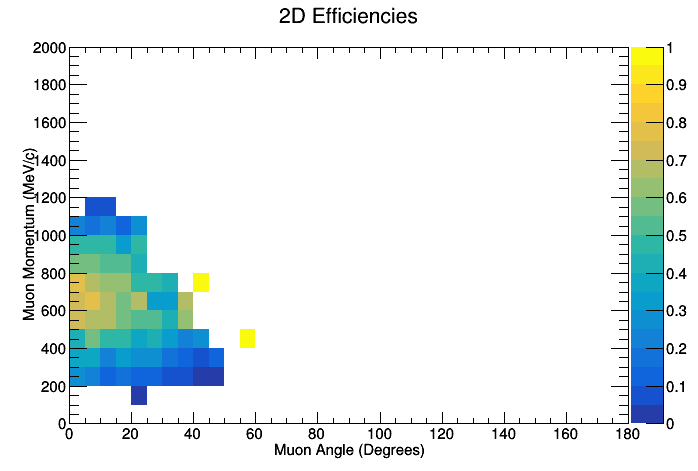
\includegraphics[width=0.6\textwidth]{CCCohPlots/2DEffANMBS.png}
\caption{Two-dimensional efficiency plot for the CC-Coh $\pi$ events of the $\bar{\nu}$-mode NEUT v5.3.6 Berger-Sehgal MC. Table \ref*{tab:app:CCCohANMBS} is the efficiency table for this two-dimensional efficiency histogram.}
\label{fig:TwoDEfficiencyCCCohANMBS}
\end{figure}


%-------------------------------------------------------------------------
\section{Conclusion}
\label{sec:conclusion}
%-------------------------------------------------------------------------

The purpose of this acceptance study was to reproduce the acceptance model that was used in SciBooNE's original study, and to see the differences that resulted from multiple CC-Coh $\pi$ models with a more modern NEUT generator (the old NEUT version originally used in the SciBooNE study is believed to be NEUT v5.0.1 and the modern version used in this study is NEUT v5.3.6). The two-dimensional efficiency histograms for CC-Inclusive events were made and are shown in Figures \ref*{fig:TwoDEfficiencyRS}-\ref*{fig:TwoDEfficiencyORS}, Figure \ref*{fig:ANMTwoDEfficiencyRS}, and Figure \ref*{fig:ANMTwoDEfficiencyBS} with the corresponding tables being Tables \ref*{tab:app:CCIncNMRS}-\ref*{tab:app:CCIncANMBS}. The two-dimensional efficiency histograms for CC-Coh $\pi$ were also made and can now be used in the re-analysis as they were intended with Figures \ref*{fig:TwoDEfficiencyCCCohNMRS}-\ref*{fig:TwoDEfficiencyCCCohNMORS}, Figure \ref*{fig:TwoDEfficiencyCCCohANMRS}, and Figure \ref*{fig:TwoDEfficiencyCCCohANMBS} being the associated CC-Coh $\pi$ two-dimensional efficiency histograms. The tables that correspond to the CC-Coh $\pi$ two-dimensional efficiency histograms are Tables \ref*{tab:app:CCCohNMRS}-\ref*{tab:app:CCCohANMBS}.

While working with CC-Inclusive events we were able to reproduce the results of a previous study, which is evident in the close agreement between the one-dimensional efficiency histograms for the muon's momentum and angle with Hiraide's thesis in Figure \ref*{fig:OneDEfficiency}. Though our model is simplistic, this agreement is a strong indication that our simplistic model is accurate and reasonable. In comparison with the two-dimensional efficiency histogram that was provided by Morgan for CC-Inclusive events, our two-dimensional efficiency histograms fail to corroborate what Morgan provided, as seen in Figures \ref*{fig:TwoDEfficiencyRS}-\ref*{fig:TwoDEfficiencyORS}. This is a result that we do not understand, but we do realize that our acceptance study is being compared with two different studies, so we do not know for certain what this implies about our acceptance study.

The results for CC-Coh $\pi$ events showed a strong difference between the Rein-Sehgal models and the Berger-Sehgal model in the four-momentum transfer variables: $|t|$, and $Q^2$ (evident in Figure \ref*{fig:NuModeCCCohGoodTAndQ2} for $\nu$-mode events and in Figure \ref*{fig:AntiNuModeCCCohGoodTAndQ2} for $\bar{\nu}$-mode events). This result has striking implications for the way that the data is sliced, but looking at the results of the two-dimensional efficiency histograms for CC-Coh $\pi$ events (Figures \ref*{fig:TwoDEfficiencyCCCohNMRS}-\ref*{fig:TwoDEfficiencyCCCohNMORS} for $\nu$-mode and Figures \ref*{fig:TwoDEfficiencyCCCohANMRS}-\ref*{fig:TwoDEfficiencyCCCohANMBS} for $\bar{\nu}$-mode) there is no clearly distinguishable difference in the two-dimensional efficiency histograms between the different models. This implies that the detector is equally sensitive to both models, and that the issue of SciBooNE's non-observance of CC-Coh $\pi$ is not a result of the detector not being sensitive to different models, but is due to the slicing of the data.

The results above strongly indicate that our simplistic model is reasonable, and they also indicate that the SciBooNE detector is equally sensitive to the different models for CC-Coh $\pi$ used in this acceptance study. This gives the clear implication that the cuts made for selecting CC-Coh $\pi$ in data are model dependent, and the selection cuts would depend on which kinematic variables are used to distinguish a CC-Coh $\pi$ event in the data. Future studies could be done on the differences in other kinematic variables between the different models, and there could also be a study that looked only at the events with a ``stopped'' muon and what their corresponding acceptance results would be.

%-------------------------------------------------------------------------

%=========================================================================
%=========================================================================
%
%=========================================================================
%=========================================================================
\newpage

\appendix


%=========================================================================
\section{Appendix: Sample Details}
\label{sec:SampleAppendix}
%=========================================================================

Appendix on samples

%-----------------------------------------------------------------------------------------------------------------|
\subsection{$\nu$-Mode Rein-Sehgal NEUTv5.3.6}
\label{sub:NMRSv5.3.6}
A sample of 1,000,000 $\nu$-mode interactions were simulated using the NEUT generator (v5.3.6) and the Rein-Sehgal model for charged-current coherent pion production. This sample correspond to the file labeled 
\begin{verbatim}
SciBooNE_numu_coh_RooTrack.root
\end{verbatim}
found at the following link (\href{https://drive.google.com/open?id=0B4rvJl9swUOxcEtpSl94RDRsc3c}{SciBooNE-MC-ROOTFiles}).

%-----------------------------------------------------------------------------------------------------------------|
\subsection{$\nu$-Mode Berger-Sehgal NEUTv5.3.6}
\label{sub:NMBSv5.3.6}
A sample of 1,000,000 $\nu$-mode interactions were simulated using the NEUT generator (v5.3.6) and the Berger-Sehgal model for charged-current coherent pion production. This sample correspond to the file labeled
\begin{verbatim}
SciBooNE_numu_coh_RooTrack_NEW.root
\end{verbatim}
found at the following link (\href{https://drive.google.com/open?id=0B4rvJl9swUOxcEtpSl94RDRsc3c}{SciBooNE-MC-ROOTFiles}).



%-----------------------------------------------------------------------------------------------------------------|
\subsection{$\nu$-Mode Rein-Sehgal NEUTv5.0.1}
\label{sub:NMRSv5.0.1}
A sample of 100,000 $\nu$-mode interactions were simulated using the NEUT generator (v5.0.1, believed to be the version used by the SciBooNE collaboration in the original publication) and the corresponding older Rein-Sehgal model for charged-current coherent pion production. This sample corresponds to the file labeled
\begin{verbatim}
SciBooNE_numu_coh_OLDNEUT_RooTrack.root
\end{verbatim}
found at the following link (\href{https://drive.google.com/open?id=0B4rvJl9swUOxcEtpSl94RDRsc3c}{SciBooNE-MC-ROOTFiles}).


%-----------------------------------------------------------------------------------------------------------------|
\subsection{$\bar{\nu}$-Mode Rein-Sehgal NEUTv5.3.6}
\label{sub:ANMRSv5.3.6}
A sample of 1,000,000 $\bar{\nu}$-mode interactions were simulated using the NEUT generator (v5.3.6) and the Rein-Sehgal model for charged-current coherent pion production. This sample corresponds to the file labeled
\begin{verbatim}
SciBooNE_numubar_coh_RooTrack.root
\end{verbatim}
found at the following link (\href{https://drive.google.com/open?id=0B4rvJl9swUOxcEtpSl94RDRsc3c}{SciBooNE-MC-ROOTFiles}).

%-----------------------------------------------------------------------------------------------------------------|
\subsection{$\bar{\nu}$-Mode Berger-Sehgal NEUTv5.3.6}
\label{sub:ANMBSv5.3.6}
A sample of 1,000,000 $\bar{\nu}$-mode interactions were simulated using the NEUT generator (v5.3.6) and the Berger-Sehgal model for charged-current coherent pion production. This sample corresponds to the file labeled
\begin{verbatim}
SciBooNE_numubar_coh_RooTrack_NEW.root
\end{verbatim}
found at the following link (\href{https://drive.google.com/open?id=0B4rvJl9swUOxcEtpSl94RDRsc3c}{SciBooNE-MC-ROOTFiles}).




%-----------------------------------------------------------------------------------------------------------------|
\subsection{Vertex Distributions}
\label{sub:vertexdistribution}
The events were all given a random initial point that was generated with the goal that the vertex distributions of this simulation would closely match the vertex distributions that Hiraide \footnote{Hiraide's thesis can be found here: \href{http://www-he.scphys.kyoto-u.ac.jp/theses/doctor/hiraide_dt.pdf}{http://www-he.scphys.kyoto-u.ac.jp/theses/doctor/hiraide\textunderscore{}dt.pdf}} showed in his thesis. This was done using the code below and a set of histograms for one of the samples is shown below the code.

\begin{lstlisting}[language=C]
TRandom3 *randX = new TRandom3();
TRandom3 *randY = new TRandom3();
TRandom3 *flat = new TRandom3();
randX->SetSeed(jentry/2);
randY->SetSeed(jentry*jentry);
flat->SetSeed(jentry*jentry*jentry);
double Xpos = randX->Gaus(1.5,1.3);
while (Xpos<0 || Xpos>3.0) { Xpos = randX->Gaus(1.5,1.3); }
double Ypos = randY->Gaus(1.5,1.05);
while (Ypos<0 || Ypos>3.0) { Ypos = randY->Gaus(1.5,1.05); }
double Zpos = flat->Uniform(0,1.7);
\end{lstlisting}


\begin{figure}[H]
\centering
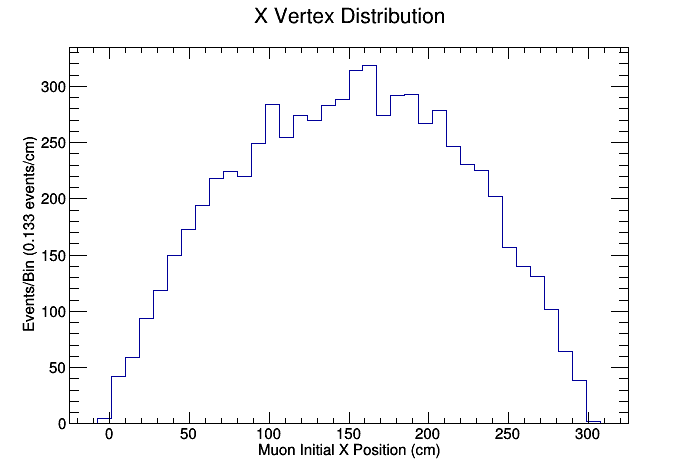
\includegraphics[width=0.3\textwidth]{NewNMReinSehgalImages/4-XVertexDistributionNMRS.png}
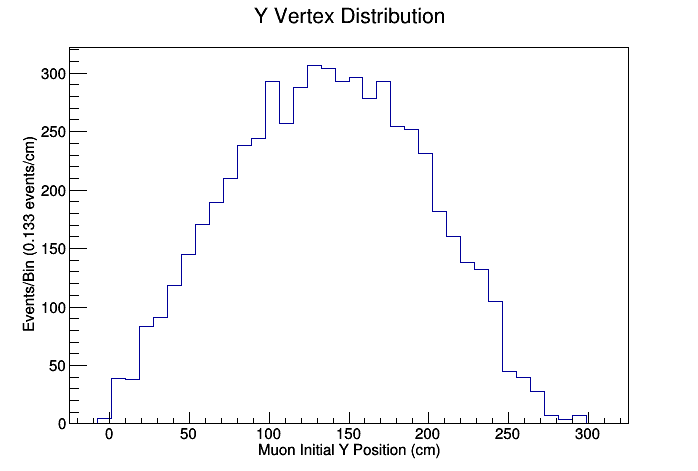
\includegraphics[width=0.3\textwidth]{NewNMReinSehgalImages/3-YVertexDistributionNMRS.png}
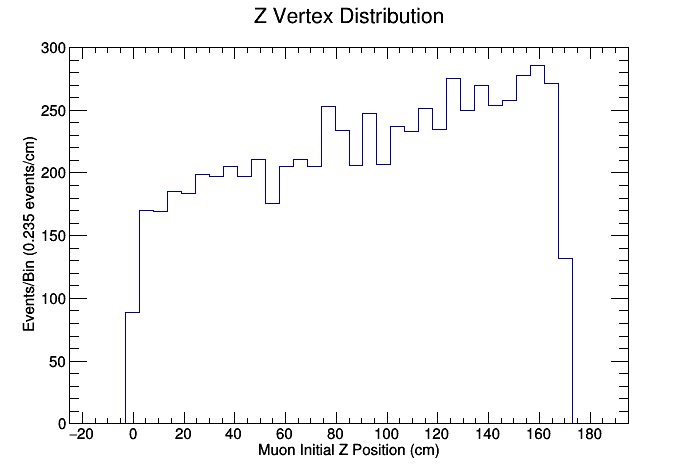
\includegraphics[width=0.3\textwidth]{NewNMReinSehgalImages/2-ZVertexDistributionNMRS.png}
\caption{Vertex distributions of the events in the $\nu$-mode NEUT v5.3.6 Rein-Sehgal sample.}
\label{fig:app:vertexdistributionRSapp}
\end{figure}





%-----------------------------------------------------------------------------------------------------------------|
\subsection{NewNMReinSehgal.C}
\label{sub:NewNMReinSehgal.C}
This file is the macro that corresponds to the "NewNMReinSehgal.h" file, which connects with this file: "SciBooNE\textunderscore numu\textunderscore coh\textunderscore RooTrack.root". This file performs the main analysis for this generated sample, and then organizes the information into many different histograms. The histograms are then written to a file titled "totalmuoninfoRS.root" inside the "ROOTFILES" directory. The "ROOTFILES" directory is included in the SciBooNE-MC repository (it is absolutely pertinent that this directory be located where the macro files are located due to how the calls of the combined data macros reference the now saved histograms). When this macro is run (which can take a while), it also plots a few different histograms. The histograms that are plotted are the ones shown in the figures below with descriptions included with the corresponding figures. The order that the histograms appear in this paper is the same order they will be shown when this macro is run in root.

\begin{figure}[H]
\centering
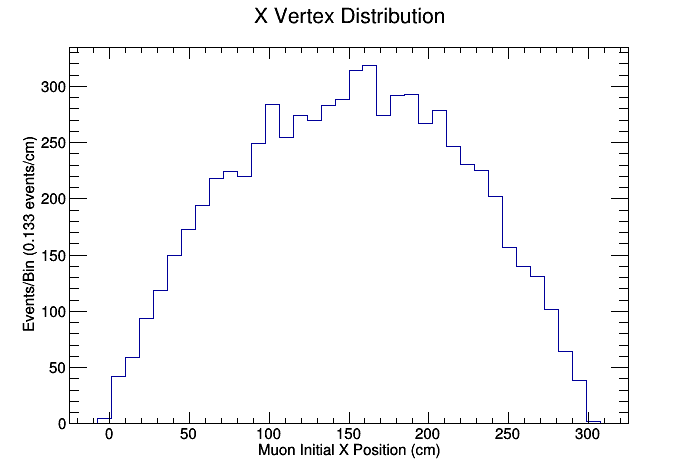
\includegraphics[width=0.3\textwidth]{NewNMReinSehgalImages/4-XVertexDistributionNMRS.png}
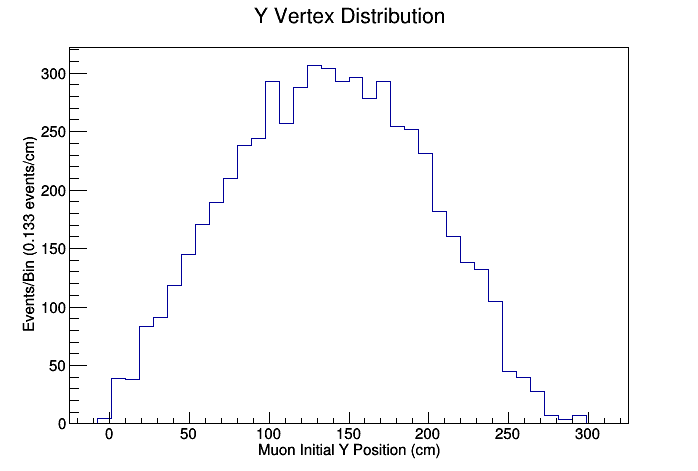
\includegraphics[width=0.3\textwidth]{NewNMReinSehgalImages/3-YVertexDistributionNMRS.png}
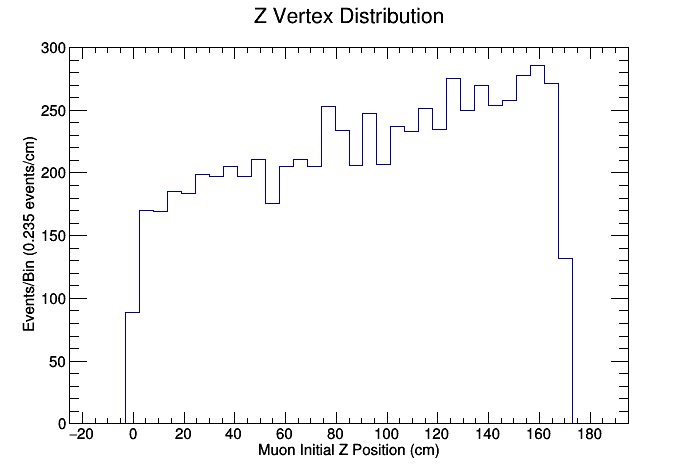
\includegraphics[width=0.3\textwidth]{NewNMReinSehgalImages/2-ZVertexDistributionNMRS.png}
\caption{Vertex distributions of the events in the $\nu$-mode NEUT v5.3.6 Rein-Sehgal sample.}
\label{fig:app:NMVertexDistributionRS}
\end{figure}

\begin{figure}[H]
\centering
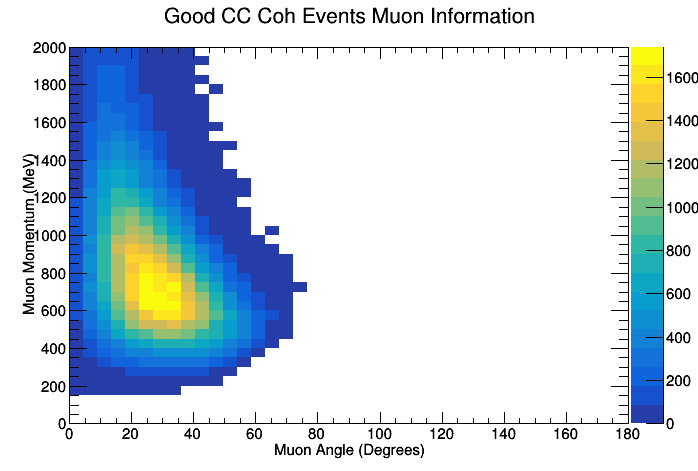
\includegraphics[width=0.4\textwidth]{NewNMReinSehgalImages/6-GoodCCCohMuonInfoNMRS.png}
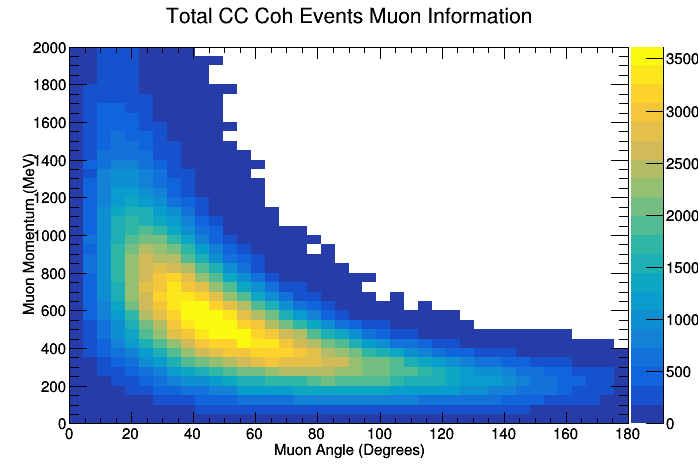
\includegraphics[width=0.4\textwidth]{NewNMReinSehgalImages/9-TotalCCCohMuonInfoNMRS.png}
\caption{These are the two-dimensional histograms that when the left is divided by the right it returns the two-dimensional efficiency histogram for the CC-Inclusive events in the NEUT v5.3.6 Rein-Sehgal sample in $\nu$ mode. The left only contains events that the muon ``stopped'' or went ``out-the-back'', penetrated the front face of the MRD, and passed through at least four layers of scinitillator before stopping. The right contains all of the events that were classified as CC-Inclusive.}
\label{fig:app:NMCCInclusiveMuon2DRS}
\end{figure}

\begin{figure}[H]
\centering
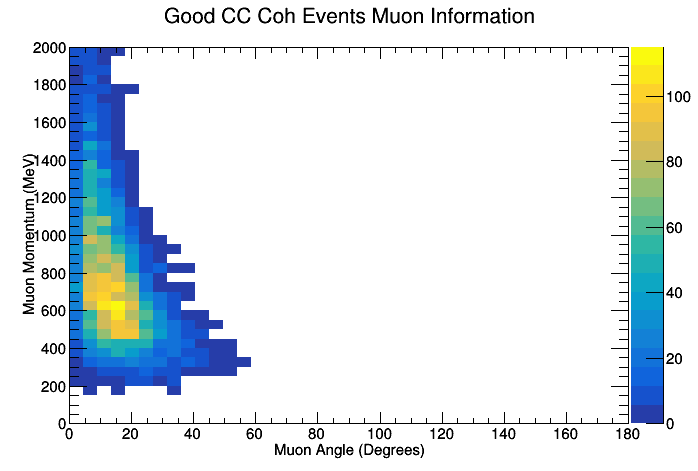
\includegraphics[width=0.4\textwidth]{NewNMReinSehgalImages/7.png}
\includegraphics[width=0.4\textwidth]{NewNMReinSehgalImages/8.png}
\caption{These are the two-dimensional histograms that when the left is divided by the right it returns the two-dimensional efficiency histogram for the CC-Coh $\pi$ events in the NEUT v5.3.6 Rein-Sehgal sample in $\nu$ mode. The left only contains events that the muon ``stopped'' or went ``out-the-back'', penetrated the front face of the MRD, and passed through at least four layers of scinitillator before stopping. The right contains all of the events that were classified as CC-Coh $\pi$.}
\label{fig:app:NMCCCohMuon2DRS}
\end{figure}

The NewNMReinSehgal.C macro also calculates many different quantities for the generated simulation of the events and saves the information in histograms that are later called upon through the plotting macros (which are after all of the analysis macros). The first quantity that is calculated for the different vertexes is the momentum of both the muon and the pion, which are both calculated using the equations:

\begin{equation}
|\vec{p}_\mu| = \sqrt{P_{\mu_x}^2 + P_{\mu_y}^2 + P_{\mu_z}^2}
\end{equation}

\begin{equation}
|\vec{p}_\pi| = \sqrt{P_{\pi_x}^2 + P_{\pi_y}^2 + P_{\pi_z}^2}
\end{equation}

\noindent
The momentum is reported in units of $MeV/c$.

The next quantity that is calculated in the macro is the angle from the beam-direction for both the muon and the pion, which are labeled as either $\theta_\mu$, or $\theta_\pi$, respectively. The angle from the beam-direction is the same as the angle from the z-direction, and this angle is known as the azimuthal angle in spherical coordinates. The calculation of the azimuthal angle is slightly more involved than the simple calculation used for finding the magnitude of the momentum of the two particles, and is calculated using the equations:

\begin{equation}
\theta_\mu = tan^{-1}(\sqrt{P_{\mu_x}^2 + P_{\mu_y}^2}/{P_{\mu_z}})
\end{equation}

\begin{equation}
\theta_\pi = tan^{-1}(\sqrt{P_{\pi_x}^2 + P_{\pi_y}^2}/{P_{\pi_z}})
\end{equation}

\noindent
The angles are reported in units of $\degree$, and should run from $0\degree$ to $180\degree$.

The last two quantities that this analysis macro calculates are the two different types of four-momentum transfers specific to this interaction, which are $Q^2$ and $|t|$. The $Q^2$ corresponds to the four-momentum transfer from the neutrino and muon to the nucleus and pion, and is calculated using the equation:

\begin{equation}
Q^2 = |(P_{\nu_\mu} - P_\mu)^2|
\end{equation}

\noindent
This equation is the four-momentum notational form. The code follows the equation below in order to compute $Q^2$:

\begin{equation}
Q^2 = |(P_{\nu_{\mu,x}} - P_{\mu_x})^2 + (P_{\nu_{\mu,y}} - P_{\mu_y})^2 + (P_{\nu_{\mu,z}} - P_{\mu_z})^2 + (P_{\nu_{\mu,E}} - P_{\mu_E})^2|
\end{equation}

\noindent
$Q^2$ is reported in units of $(MeV/c)^2$.

The $|t|$ corresponds to the four-momentum transfer from the neutrino, muon, and pion to the nucleus, and is calculated using the equation:

\begin{equation}
|t| = |(Q - P_\pi)^2| = |(P_{\nu_\mu} - P_\mu - P_\pi)^2|
\end{equation}

\noindent
This equation is the four-momentum notational form. The code follows the equation below in order to compute $|t|$:

\begin{equation}
|t| = |(P_{\nu_{\mu,x}} - P_{\mu_x} - P_{\pi_x})^2 + (P_{\nu_{\mu,y}} - P_{\mu_y} - P_{\pi_y})^2 + (P_{\nu_{\mu,z}} - P_{\mu_z} - P_{\pi_z})^2 + (P_{\nu_{\mu,E}} - P_{\mu_E} - P_{\pi_E})^2|
\end{equation}

\noindent
$|t|$ is reported in units of $(MeV/c)^2$.

%-----------------------------------------------------------------------------------------------------------------|
\subsection{NewNMBergerSehgal.C}
\label{sub:NewNMBergerSehgal.C}
This file is the macro that corresponds to the "NewNMBergerSehgal.h" file, which connects with this file: "SciBooNE\textunderscore numu\textunderscore coh\textunderscore RooTrack\textunderscore NEW.root". This file performs the main analysis for this generated sample, and then organizes the information into many different histograms. The histograms are then written to a file titled "totalmuoninfoBS.root" inside the "ROOTFILES" directory. The "ROOTFILES" directory is included in the SciBooNE-MC repository (it is absolutely pertinent that this directory be located where the macro files are located due to how the calls of the combined data macros reference the now saved histograms).

\begin{figure}[H]
\centering
\includegraphics[width=0.3\textwidth]{NewNMBergerSehgalImages/4-XVertexDistributionNMBS.png}
\includegraphics[width=0.3\textwidth]{NewNMBergerSehgalImages/3-YVertexDistributionNMBS.png}
\includegraphics[width=0.3\textwidth]{NewNMBergerSehgalImages/2-ZVertexDistributionNMBS.png}
\caption{Vertex distributions of the events in the $\nu$-mode NEUT v5.3.6 Berger-Sehgal sample.}
\label{fig:app:NMVertexDistributionBS}
\end{figure}

\begin{figure}[H]
\centering
\includegraphics[width=0.4\textwidth]{NewNMBergerSehgalImages/6-GoodCCCohMuonInfoNMBS.png}
\includegraphics[width=0.4\textwidth]{NewNMBergerSehgalImages/9-TotalCCCohMuonInfoNMBS.png}
\caption{These are the two-dimensional histograms that when the left is divided by the right it returns the two-dimensional efficiency histogram for the CC-Inclusive events in the NEUT v5.3.6 Berger-Sehgal sample in $\nu$ mode. The left only contains events that the muon ``stopped'' or went ``out-the-back'', penetrated the front face of the MRD, and passed through at least four layers of scinitillator before stopping. The right contains all of the events that were classified as CC-Inclusive.}
\label{fig:app:NMCCInclusiveMuon2DBS}
\end{figure}

\begin{figure}[H]
\centering
\includegraphics[width=0.4\textwidth]{NewNMBergerSehgalImages/7.png}
\includegraphics[width=0.4\textwidth]{NewNMBergerSehgalImages/8.png}
\caption{These are the two-dimensional histograms that when the left is divided by the right it returns the two-dimensional efficiency histogram for the CC-Coh $\pi$ events in the NEUT v5.3.6 Berger-Sehgal sample in $\nu$ mode. The left only contains events that the muon ``stopped'' or went ``out-the-back'', penetrated the front face of the MRD, and passed through at least four layers of scinitillator before stopping. The right contains all of the events that were classified as CC-Coh $\pi$.}
\label{fig:app:NMCCCohMuon2DBS}
\end{figure}


%-----------------------------------------------------------------------------------------------------------------|
\subsection{OldNMReinSehgal.C}
\label{sub:OldNMReinSehgal.C}
This file is the macro that corresponds to the "OldNMReinSehgal.h" file, which connects with this file: "SciBooNE\textunderscore numu\textunderscore coh\textunderscore OLDNEUT\textunderscore RooTrack.root". This file performs the main analysis for this generated sample, and then organizes the information into many different histograms. The histograms are then written to a file titled "totalmuoninfoOBS.root" inside the "ROOTFILES" directory. The "ROOTFILES" directory is included in the SciBooNE-MC repository (it is absolutely pertinent that this directory be located where the macro files are located due to how the calls of the combined data macros reference the now saved histograms).

\begin{figure}[H]
\centering
\includegraphics[width=0.3\textwidth]{OldNMReinSehgalImages/4-XVertexDistributionNMORS.png}
\includegraphics[width=0.3\textwidth]{OldNMReinSehgalImages/3-YVertexDistributionNMORS.png}
\includegraphics[width=0.3\textwidth]{OldNMReinSehgalImages/2-ZVertexDistributionNMORS.png}
\caption{Vertex distributions of the events in the $\nu$-mode NEUT v5.0.1 Rein-Sehgal sample.}
\label{fig:app:NMVertexDistributionORS}
\end{figure}

\begin{figure}[H]
\centering
\includegraphics[width=0.4\textwidth]{OldNMReinSehgalImages/6-GoodCCCohMuonInfoNMORS.png}
\includegraphics[width=0.4\textwidth]{OldNMReinSehgalImages/9-TotalCCCohMuonInfoNMORS.png}
\caption{These are the two-dimensional histograms that when the left is divided by the right it returns the two-dimensional efficiency histogram for the CC-Inclusive events in the NEUT v5.0.1 Rein-Sehgal sample in $\nu$ mode. The left only contains events that the muon ``stopped'' or went ``out-the-back'', penetrated the front face of the MRD, and passed through at least four layers of scinitillator before stopping. The right contains all of the events that were classified as CC-Inclusive.}
\label{fig:app:NMCCInclusiveMuon2DORS}
\end{figure}

\begin{figure}[H]
\centering
\includegraphics[width=0.4\textwidth]{OldNMReinSehgalImages/7.png}
\includegraphics[width=0.4\textwidth]{OldNMReinSehgalImages/8.png}
\caption{These are the two-dimensional histograms that when the left is divided by the right it returns the two-dimensional efficiency histogram for the CC-Coh $\pi$ events in the NEUT v5.0.1 Rein-Sehgal sample in $\nu$ mode. The left only contains events that the muon ``stopped'' or went ``out-the-back'', penetrated the front face of the MRD, and passed through at least four layers of scinitillator before stopping. The right contains all of the events that were classified as CC-Coh $\pi$.}
\label{fig:app:NMCCCohMuon2DORS}
\end{figure}


%-----------------------------------------------------------------------------------------------------------------|
\subsection{NewANMReinSehgal.C}
\label{sub:NewANMReinSehgal.C}
This file is the macro that corresponds to the "NewANMReinSehgal.h" file, which connects with this file: "SciBooNE\textunderscore numubar\textunderscore coh\textunderscore RooTrack.root". This file performs the main analysis for this generated sample, and then organizes the information into many different histograms. The histograms are then written to a file titled "totalmuoninfoRSBar.root" inside the "ROOTFILES" directory. The "ROOTFILES" directory is included in the SciBooNE-MC repository (it is absolutely pertinent that this directory be located where the macro files are located due to how the calls of the combined data macros reference the now saved histograms).

\begin{figure}[H]
\centering
\includegraphics[width=0.3\textwidth]{NewANMReinSehgalImages/4-XVertexDistributionANMRS.png}
\includegraphics[width=0.3\textwidth]{NewANMReinSehgalImages/3-YVertexDistributionANMRS.png}
\includegraphics[width=0.3\textwidth]{NewANMReinSehgalImages/2-ZVertexDistributionANMRS.png}
\caption{Vertex distributions of the events in the $\bar{\nu}$-mode NEUT v5.3.6 Rein-Sehgal sample.}
\label{fig:app:ANMVertexDistributionRS}
\end{figure}

\begin{figure}[H]
\centering
\includegraphics[width=0.4\textwidth]{NewANMReinSehgalImages/6-GoodCCCohMuonInfoANMRS.png}
\includegraphics[width=0.4\textwidth]{NewANMReinSehgalImages/9-TotalCCCohMuonInfoANMRS.png}
\caption{These are the two-dimensional histograms that when the left is divided by the right it returns the two-dimensional efficiency histogram for the CC-Inclusive events in the NEUT v5.3.6 Rein-Sehgal sample in $\bar{\nu}$ mode. The left only contains events that the muon ``stopped'' or went ``out-the-back'', penetrated the front face of the MRD, and passed through at least four layers of scinitillator before stopping. The right contains all of the events that were classified as CC-Inclusive.}
\label{fig:app:ANMCCInclusiveMuon2DRS}
\end{figure}

\begin{figure}[H]
\centering
\includegraphics[width=0.4\textwidth]{NewANMReinSehgalImages/7.png}
\includegraphics[width=0.4\textwidth]{NewANMReinSehgalImages/8.png}
\caption{These are the two-dimensional histograms that when the left is divided by the right it returns the two-dimensional efficiency histogram for the CC-Coh $\pi$ events in the NEUT v5.3.6 Rein-Sehgal sample in $\bar{\nu}$ mode. The left only contains events that the muon ``stopped'' or went ``out-the-back'', penetrated the front face of the MRD, and passed through at least four layers of scinitillator before stopping. The right contains all of the events that were classified as CC-Coh $\pi$.}
\label{fig:app:ANMCCCohMuon2DRS}
\end{figure}


%-----------------------------------------------------------------------------------------------------------------|
\subsection{NewANMBergerSehgal.C}
\label{sub:NewANMBergerSehgal.C}
This file is the macro that corresponds to the "NewANMBergerSehgal.h" file, which connects with this file: "SciBooNE\textunderscore numubar\textunderscore coh\textunderscore RooTrack\textunderscore NEW.root". This file performs the main analysis for this generated sample, and then organizes the information into many different histograms. The histograms are then written to a file titled "totalmuoninfoBSBar.root" inside the "ROOTFILES" directory. The "ROOTFILES" directory is included in the SciBooNE-MC repository (it is absolutely pertinent that this directory be located where the macro files are located due to how the calls of the combined data macros reference the now saved histograms).


\begin{figure}[H]
\centering
\includegraphics[width=0.3\textwidth]{NewANMBergerSehgalImages/4-XVertexDistributionANMBS.png}
\includegraphics[width=0.3\textwidth]{NewANMBergerSehgalImages/3-YVertexDistributionANMBS.png}
\includegraphics[width=0.3\textwidth]{NewANMBergerSehgalImages/2-ZVertexDistributionANMBS.png}
\caption{Vertex distributions of the events in the $\bar{\nu}$-mode NEUT v5.3.6 Berger-Sehgal sample.}
\label{fig:app:ANMVertexDistributionBS}
\end{figure}

\begin{figure}[H]
\centering
\includegraphics[width=0.4\textwidth]{NewANMBergerSehgalImages/6-GoodCCCohMuonInfoANMBS.png}
\includegraphics[width=0.4\textwidth]{NewANMBergerSehgalImages/9-TotalCCCohMuonInfoANMBS.png}
\caption{These are the two-dimensional histograms that when the left is divided by the right it returns the two-dimensional efficiency histogram for the CC-Inclusive events in the NEUT v5.3.6 Berger-Sehgal sample in $\bar{\nu}$ mode. The left only contains events that the muon ``stopped'' or went ``out-the-back'', penetrated the front face of the MRD, and passed through at least four layers of scinitillator before stopping. The right contains all of the events that were classified as CC-Inclusive.}
\label{fig:app:ANMCCInclusiveMuon2DBS}
\end{figure}

\begin{figure}[H]
\centering
\includegraphics[width=0.4\textwidth]{NewANMBergerSehgalImages/7.png}
\includegraphics[width=0.4\textwidth]{NewANMBergerSehgalImages/8.png}
\caption{These are the two-dimensional histograms that when the left is divided by the right it returns the two-dimensional efficiency histogram for the CC-Coh $\pi$ events in the NEUT v5.3.6 Berger-Sehgal sample in $\bar{\nu}$ mode. The left only contains events that the muon ``stopped'' or went ``out-the-back'', penetrated the front face of the MRD, and passed through at least four layers of scinitillator before stopping. The right contains all of the events that were classified as CC-Coh $\pi$.}
\label{fig:app:ANMCCCohMuon2DBS}
\end{figure}


%-----------------------------------------------------------------------------------------------------------------|
\subsection{NMCombinedPlots.C}
\label{sub:NMCombinedPlots.C}
This is the file that performs the main plotting operations for the $\nu$-mode samples using the muon's information. All of the muon efficiency plots for $\nu$-mode are made with this file.

\begin{figure}[H]
\centering
\includegraphics[width=0.4\textwidth]{NMCombinedPlotsImages/22-NMCombinedPlots.png}
\includegraphics[width=0.4\textwidth]{NMCombinedPlotsImages/23-NMCombinedPlots.png}
\caption{These are the $\nu$-mode one-dimensional efficiency plots of the muon information for CC-Inclusive events. The left is the angle efficiency plot and the right is the momentum efficiency plot for the muon in all three $\nu$-mode samples.}
\label{fig:app:NMCCInclusive1DEff}
\end{figure}

\begin{figure}[H]
\centering
\includegraphics[width=0.6\textwidth]{CCInclusivePlots/2DEffCompareNMRS.png}
\caption{Two-dimensional efficiency plot for the $\nu$-mode NEUT v5.3.6 Rein-Sehgal CC-Inclusive sample.}
\label{fig:app:NMCCInclusiveMuon2DEffRS}
\end{figure}

\begin{figure}[H]
\centering
\includegraphics[width=0.6\textwidth]{CCInclusivePlots/2DEffCompareNMBS.png}
\caption{Two-dimensional efficiency plot for the $\nu$-mode NEUT v5.3.6 Berger-Sehgal CC-Inclusive sample.}
\label{fig:app:NMCCInclusiveMuon2DEffBS}
\end{figure}

\begin{figure}[H]
\centering
\includegraphics[width=0.6\textwidth]{CCInclusivePlots/2DEffCompareNMORS.png}
\caption{Two-dimensional efficiency plot for the $\nu$-mode NEUT v5.0.1 Rein-Sehgal CC-Inclusive sample.}
\label{fig:app:NMCCInclusiveMuon2DEffORS}
\end{figure}

\begin{figure}[H]
\centering
\includegraphics[width=0.4\textwidth]{NMCombinedPlotsImages/14-NMCombinedPlots.png}
\includegraphics[width=0.4\textwidth]{NMCombinedPlotsImages/16-NMCombinedPlots.png}
\caption{These are the two plots for muon angles in $\nu$-mode that are used to make the one-dimensional efficiency plot for the angles in CC-Coh $\pi$ events. The left is the plot for the events that had a muon make it to the front face of the MRD and the muon either ``stopped'' or went ``out-the-back'' face, and penetrated at least four layers of scintillator of the MRD. The right plot is the muon angles for all of the events that were classified as CC-Coh $\pi$. The left divided by the right gives the efficiency plot for the muon angles in CC-Coh $\pi$ events for all three $\nu$-mode samples.}
\label{fig:app:NMCCCohMuonAng}
\end{figure}

\begin{figure}[H]
\centering
\includegraphics[width=0.6\textwidth]{NMCombinedPlotsImages/24-NMCombinedPlots.png}
\caption{This is the one-dimensional muon angle efficiency plot for the CC-Coh $\pi$ events from the $\nu$-mode samples.}
\label{fig:app:NMCCCohAng1DEff}
\end{figure}

\begin{figure}[H]
\centering
\includegraphics[width=0.4\textwidth]{NMCombinedPlotsImages/15-NMCombinedPlots.png}
\includegraphics[width=0.4\textwidth]{NMCombinedPlotsImages/17-NMCombinedPlots.png}
\caption{These are the two plots for muon momentums in $\nu$-mode that are used to make the one-dimensional efficiency plot for the momentums in CC-Coh $\pi$ events. The left is the plot for the events that had a muon make it to the front face of the MRD and the muon either ``stopped'' or went ``out-the-back'' face, and penetrated at least four layers of scintillator of the MRD. The right plot is the muon momentums for all of the events that were classified as CC-Coh $\pi$. The left divided by the right gives the efficiency plot for the muon momentums in CC-Coh $\pi$ events for all three $\nu$-mode samples.}
\label{fig:app:NMCCCohMuonMom}
\end{figure}

\begin{figure}[H]
\centering
\includegraphics[width=0.6\textwidth]{NMCombinedPlotsImages/25-NMCombinedPlots.png}
\caption{This is the one-dimensional muon momentum efficiency plot for the CC-Coh $\pi$ events from the $\nu$-mode samples.}
\label{fig:app:NMCCCohMom1DEff}
\end{figure}

\begin{figure}[H]
\centering
\includegraphics[width=0.6\textwidth]{CCCohPlots/2DEffNMRS.png}
\caption{Two-dimensional efficiency plot for the $\nu$-mode NEUT v5.3.6 Rein-Sehgal CC-Coh $\pi$ sample.}
\label{fig:app:NMCCCohMuon2DEffRS}
\end{figure}

\begin{figure}[H]
\centering
\includegraphics[width=0.6\textwidth]{CCCohPlots/2DEffNMBS.png}
\caption{Two-dimensional efficiency plot for the $\nu$-mode NEUT v5.3.6 Berger-Sehgal CC-Coh $\pi$ sample.}
\label{fig:app:NMCCCohMuon2DEffBS}
\end{figure}

\begin{figure}[H]
\centering
\includegraphics[width=0.6\textwidth]{CCCohPlots/2DEffNMORS.png}
\caption{Two-dimensional efficiency plot for the $\nu$-mode NEUT v5.0.1 Rein-Sehgal CC-Coh $\pi$ sample.}
\label{fig:app:NMCCCohMuon2DEffORS}
\end{figure}

%-----------------------------------------------------------------------------------------------------------------|
\subsection{NMPionPlotting.C}
\label{sub:NMPionPlotting.C}
This is the file that performs the main plotting operations for the $\nu$-mode samples using the pion's information. All of the combined pion plots for $\nu$-mode are made with this file.

\begin{figure}[H]
\centering
\includegraphics[width=0.4\textwidth]{NMPionPlottingImages/7-NMPionPlotting.png}
\includegraphics[width=0.4\textwidth]{NMPionPlottingImages/10-NMPionPlotting.png}
\caption{These are the angles of the pions in CC-Coh $\pi$ events in the $\nu$-mode samples. The left plot is the angles for the pions where the muon made it to the MRD and either ``stopped'' or went ``out-the-back'' face of the MRD, and penetrated four layers of scintillator of the MRD for all three $\nu$-mode samples. The right plot is the pion angles for all of the events that were classified as CC-Coh $\pi$ for the three $\nu$-mode samples.}
\label{fig:app:NMPionAng}
\end{figure}

\begin{figure}[H]
\centering
\includegraphics[width=0.4\textwidth]{NMPionPlottingImages/8-NMPionPlotting.png}
\includegraphics[width=0.4\textwidth]{NMPionPlottingImages/11-NMPionPlotting.png}
\caption{These are the momentums of the pions in CC-Coh $\pi$ events in the $\nu$-mode samples. The left plot is the momentums for the pions where the muon made it to the MRD and either ``stopped'' or went ``out-the-back'' face of the MRD, and penetrated four layers of scintillator of the MRD for all three $\nu$-mode samples. The right plot is the pion momentums for all of the events that were classified as CC-Coh $\pi$ for the three $\nu$-mode samples.}
\label{fig:app:NMPionMom}
\end{figure}

\begin{figure}[H]
\centering
\includegraphics[width=0.4\textwidth]{NMPionPlottingImages/9-NMPionPlotting.png}
\includegraphics[width=0.4\textwidth]{NMPionPlottingImages/12-NMPionPlotting.png}
\caption{These are the energies of the pions in CC-Coh $\pi$ events in the $\nu$-mode samples. The left plot is the energies for the pions where the muon made it to the MRD and either ``stopped'' or went ``out-the-back'' face of the MRD, and penetrated four layers of scintillator of the MRD for all three $\nu$-mode samples. The right plot is the pion energies for all of the events that were classified as CC-Coh $\pi$ for the three $\nu$-mode samples.}
\label{fig:app:NMPionEnergy}
\end{figure}

%-----------------------------------------------------------------------------------------------------------------|
\subsection{NMFourSquaredPlotting.C}
\label{sub:NMFourSquaredPlotting.C}
All of the four-momentum transfer (both $|t|$ and $Q^2$) combined plots are made with this file for $\nu$-mode.

\begin{figure}[H]
\centering
\includegraphics[width=0.4\textwidth]{CCCohPlots/NMCCCohGoodT.png}
\includegraphics[width=0.4\textwidth]{CCCohPlots/NMCCCohGoodQ2.png}
\caption{The $|t|$ momentum transfer for the ``stopped'' and the ``out-the-back'' events (left) and $Q^2$ momentum transfer for the ``stopped'' and the ``out-the-back'' events (right) for $\nu$-mode CC-Coh $\pi$ interactions for the three models included in this study.}
\label{fig:app:NMTQ2}
\end{figure}

%-----------------------------------------------------------------------------------------------------------------|
\subsection{ANMCombinedPlots.C}
\label{sub:ANMCombinedPlots.C}
This is the file that performs the main plotting operations for the $\bar{\nu}$-mode samples using the muon's information. All of the muon efficiency plots for $\bar{\nu}$-mode are made with this file.

\begin{figure}[H]
\centering
\includegraphics[width=0.4\textwidth]{ANMCombinedPlotsImages/15-ANMCombinedPlots.png}
\includegraphics[width=0.4\textwidth]{ANMCombinedPlotsImages/16-ANMCombinedPlots.png}
\caption{These are the $\bar{\nu}$-mode one-dimensional efficiency plots of the muon information for CC-Inclusive events. The left is the angle efficiency plot and the right is the momentum efficiency plot for the muon in both $\bar{\nu}$-mode samples.}
\label{fig:app:ANMCCInclusive1DEff}
\end{figure}

\begin{figure}[H]
\centering
\includegraphics[width=0.6\textwidth]{CCInclusivePlots/2DEffCompareANMRS.png}
\caption{Two-dimensional efficiency plot for the $\bar{\nu}$-mode NEUT v5.3.6 Rein-Sehgal CC-Inclusive sample.}
\label{fig:app:ANMCCInclusiveMuon2DEffRS}
\end{figure}

\begin{figure}[H]
\centering
\includegraphics[width=0.6\textwidth]{CCInclusivePlots/2DEffCompareANMBS.png}
\caption{Two-dimensional efficiency plot for the $\bar{\nu}$-mode NEUT v5.3.6 Berger-Sehgal CC-Inclusive sample.}
\label{fig:app:ANMCCInclusiveMuon2DEffBS}
\end{figure}

\begin{figure}[H]
\centering
\includegraphics[width=0.4\textwidth]{ANMCombinedPlotsImages/11-ANMCombinedPlots.png}
\includegraphics[width=0.4\textwidth]{ANMCombinedPlotsImages/13-ANMCombinedPlots.png}
\caption{These are the two plots for muon angles in $\bar{\nu}$-mode that are used to make the one-dimensional efficiency plot for the angles in CC-Coh $\pi$ events. The left is the plot for the events that had a muon make it to the front face of the MRD and the muon either ``stopped'' or went ``out-the-back'' face, and penetrated at least four layers of scintillator of the MRD. The right plot is the muon angles for all of the events that were classified as CC-Coh $\pi$. The left divided by the right gives the efficiency plot for the muon angles in CC-Coh $\pi$ events for both $\bar{\nu}$-mode samples.}
\label{fig:app:ANMCCCohMuonAng}
\end{figure}

\begin{figure}[H]
\centering
\includegraphics[width=0.6\textwidth]{ANMCombinedPlotsImages/17-ANMCombinedPlots.png}
\caption{This is the one-dimensional muon angle efficiency plot for the CC-Coh $\pi$ events from the $\bar{\nu}$-mode samples.}
\label{fig:app:ANMCCCohAng1DEff}
\end{figure}

\begin{figure}[H]
\centering
\includegraphics[width=0.4\textwidth]{ANMCombinedPlotsImages/12-ANMCombinedPlots.png}
\includegraphics[width=0.4\textwidth]{ANMCombinedPlotsImages/14-ANMCombinedPlots.png}
\caption{These are the two plots for muon momentums in $\bar{\nu}$-mode that are used to make the one-dimensional efficiency plot for the momentums in CC-Coh $\pi$ events. The left is the plot for the events that had a muon make it to the front face of the MRD and the muon either ``stopped'' or went ``out-the-back'' face, and penetrated at least four layers of scintillator of the MRD. The right plot is the muon momentums for all of the events that were classified as CC-Coh $\pi$. The left divided by the right gives the efficiency plot for the muon momentums in CC-Coh $\pi$ events for both $\bar{\nu}$-mode samples.}
\label{fig:app:ANMCCCohMuonMom}
\end{figure}

\begin{figure}[H]
\centering
\includegraphics[width=0.6\textwidth]{ANMCombinedPlotsImages/18-ANMCombinedPlots.png}
\caption{This is the one-dimensional muon momentum efficiency plot for the CC-Coh $\pi$ events from the $\bar{\nu}$-mode samples.}
\label{fig:app:ANMCCCohMom1DEff}
\end{figure}

\begin{figure}[H]
\centering
\includegraphics[width=0.6\textwidth]{CCCohPlots/2DEffANMRS.png}
\caption{Two-dimensional efficiency plot for the $\bar{\nu}$-mode NEUT v5.3.6 Rein-Sehgal CC-Coh $\pi$ sample.}
\label{fig:app:ANMCCCohMuon2DEffRS}
\end{figure}

\begin{figure}[H]
\centering
\includegraphics[width=0.6\textwidth]{CCCohPlots/2DEffANMBS.png}
\caption{Two-dimensional efficiency plot for the $\bar{\nu}$-mode NEUT v5.3.6 Berger-Sehgal CC-Coh $\pi$ sample.}
\label{fig:app:ANMCCCohMuon2DEffBS}
\end{figure}

%-----------------------------------------------------------------------------------------------------------------|
\subsection{ANMPionPlotting.C}
\label{sub:ANMPionPlotting.C}
This is the file that performs the main plotting operations for the $\nu$-mode samples using the pion's information. All of the combined pion plots for $\nu$-mode are made with this file.

\begin{figure}[H]
\centering
\includegraphics[width=0.4\textwidth]{ANMPionPlottingImages/7-ANMPionPlotting.png}
\includegraphics[width=0.4\textwidth]{ANMPionPlottingImages/10-ANMPionPlotting.png}
\caption{These are the angles of the pions in CC-Coh $\pi$ events in the $\bar{\nu}$-mode samples. The left plot is the angles for the pions where the muon made it to the MRD and either ``stopped'' or went ``out-the-back'' face of the MRD, and penetrated four layers of scintillator of the MRD for both $\bar{\nu}$-mode samples. The right plot is the pion angles for all of the events that were classified as CC-Coh $\pi$ for both $\bar{\nu}$-mode samples.}
\label{fig:app:ANMPionAng}
\end{figure}

\begin{figure}[H]
\centering
\includegraphics[width=0.4\textwidth]{ANMPionPlottingImages/8-ANMPionPlotting.png}
\includegraphics[width=0.4\textwidth]{ANMPionPlottingImages/11-ANMPionPlotting.png}
\caption{These are the momentums of the pions in CC-Coh $\pi$ events in the $\bar{\nu}$-mode samples. The left plot is the momentums for the pions where the muon made it to the MRD and either ``stopped'' or went ``out-the-back'' face of the MRD, and penetrated four layers of scintillator of the MRD for both $\bar{\nu}$-mode samples. The right plot is the pion momentums for all of the events that were classified as CC-Coh $\pi$ for both $\bar{\nu}$-mode samples.}
\label{fig:app:ANMPionMom}
\end{figure}

\begin{figure}[H]
\centering
\includegraphics[width=0.4\textwidth]{ANMPionPlottingImages/9-ANMPionPlotting.png}
\includegraphics[width=0.4\textwidth]{ANMPionPlottingImages/12-ANMPionPlotting.png}
\caption{These are the energies of the pions in CC-Coh $\pi$ events in the $\bar{\nu}$-mode samples. The left plot is the energies for the pions where the muon made it to the MRD and either ``stopped'' or went ``out-the-back'' face of the MRD, and penetrated four layers of scintillator of the MRD for both $\bar{\nu}$-mode samples. The right plot is the pion energies for all of the events that were classified as CC-Coh $\pi$ for both $\bar{\nu}$-mode samples.}
\label{fig:app:ANMPionEnergy}
\end{figure}

%-----------------------------------------------------------------------------------------------------------------|
\subsection{ANMFourSquaredPlotting.C}
\label{sub:ANMFourSquaredPlotting.C}
All of the four-momentum transfer (both $|t|$ and $Q^2$) combined plots are made with this file for $\bar{\nu}$-mode.

\begin{figure}[H]
\centering
\includegraphics[width=0.4\textwidth]{CCCohPlots/ANMCCCohGoodT.png}
\includegraphics[width=0.4\textwidth]{CCCohPlots/ANMCCCohGoodQ2.png}
\caption{The $|t|$ momentum transfer for the ``stopped'' and the ``out-the-back'' events (left) and $Q^2$ momentum transfer for the ``stopped'' and the ``out-the-back'' events (right) for $\bar{\nu}$-mode CC-Coh $\pi$ interactions for both models included in this study.}
\label{fig:app:ANMTQ2}
\end{figure}
%%%%%%%%%%%%%%%%%%%%%%%%%%%%%%%% The Files and Their Outputs section ends here! %%%%%%%%%%%%%%%%%%%%%%%%%%%%%%%%%|



%======================================== A New Section Begins Here =============================================|
%\section{Steps for Running the Code}
%The instructions on how to run the code and the order the files need to run in so that there are no resulting error messages, or other issues while running the code, are detailed in this section.
%
%\begin{adjustwidth}{4.0em}{0pt}
%\begin{steps}
%  \item This is the first step. (Run the NewNM macros and the NewANM macros and the OldNM macro.)
%  \item This is the second step. (Run the combined plotting macros.)
%  \item This is the third step. (Run the Pion Plotting macros.)
%  \item Etc. (Run the FourSquaredMomentum macros.)
%\end{steps}
%\end{adjustwidth}
%%%%%%%%%%%%%%%%%%%%%%%%%%%%%% The Steps for Running the Code section ends here! %%%%%%%%%%%%%%%%%%%%%%%%%%%%%%%|


%===================================== A New Section Begins Here ===============================================|
\section{Efficiency Tables}
\label{sec:EffTab}

This is the section of the appendix that contains the efficiency tables of the two-dimensional histograms that were seen throughout the technical note. This section is broken into two subsections: one for the CC-Inclusive two-dimensional efficiency histograms, and the other for the CC-Coh $\pi$ two-dimensional efficiency histograms.

\subsection{Charged-Current Inclusive Sample Efficiency Tables}
\label{sub:CCInclusiveEffTab}

These are the corresponding tables to the 2D Efficiency histograms for CC-Inclusive events.

\newpage
\begin{landscape}
\begin{table}
\centering
\caption{Efficiency Table of 2D Histogram for $\nu$-mode CC-Inclusive NEUT v5.3.6 Rein-Sehgal}
\label{tab:app:CCIncNMRS}
\begin{adjustbox}{width=\paperwidth}
\csvautotabular{TechNoteTables/New-NM-RS.csv}
\end{adjustbox}
\end{table}
\end{landscape}

\newpage
\begin{landscape}
\begin{table}
\centering
\caption{Efficiency Table of 2D Histogram for $\nu$-mode CC-Inclusive NEUT v5.3.6 Berger-Sehgal}
\label{tab:app:CCIncNMBS}
\begin{adjustbox}{width=\paperwidth}
\csvautotabular{TechNoteTables/New-NM-BS.csv}
\end{adjustbox}
\end{table}
\end{landscape}

\newpage
\begin{landscape}
\begin{table}
\centering
\caption{Efficiency Table of 2D Histogram for $\nu$-mode CC-Inclusive NEUT v5.0.1 Rein-Sehgal}
\label{tab:app:CCIncNMORS}
\begin{adjustbox}{width=\paperwidth}
\csvautotabular{TechNoteTables/Old-NM-RS.csv}
\end{adjustbox}
\end{table}
\end{landscape}

\newpage
\begin{landscape}
\begin{table}
\centering
\caption{Efficiency Table of 2D Histogram for $\bar{\nu}$-mode CC-Inclusive NEUT v5.3.6 Rein-Sehgal}
\label{tab:app:CCIncANMRS}
\begin{adjustbox}{width=\paperwidth}
\csvautotabular{TechNoteTables/New-ANM-RS.csv}
\end{adjustbox}
\end{table}
\end{landscape}

\newpage
\begin{landscape}
\begin{table}
\centering
\caption{Efficiency Table of 2D Histogram for $\bar{\nu}$-mode CC-Inclusive NEUT v5.3.6 Berger-Sehgal}
\label{tab:app:CCIncANMBS}
\begin{adjustbox}{width=\paperwidth}
\csvautotabular{TechNoteTables/New-ANM-BS.csv}
\end{adjustbox}
\end{table}
\end{landscape}



\subsection{Charged-Current Coherent Pion Production Efficiency Tables}
\label{sub:CCCohEffTab}

These are the corresponding tables to the 2D Efficiency histograms for CC-Coh $\pi$ events.

\newpage
\begin{landscape}
\begin{table}
\centering
\caption{Efficiency Table of 2D Histogram for $\nu$-mode CC-Coh $\pi$ NEUT v5.3.6 Rein-Sehgal}
\label{tab:app:CCCohNMRS}
\begin{adjustbox}{width=\paperwidth}
\csvautotabular{TechNoteTables/CC-Coh-New-NM-RS.csv}
\end{adjustbox}
\end{table}
\end{landscape}

\newpage
\begin{landscape}
\begin{table}
\centering
\caption{Efficiency Table of 2D Histogram for $\nu$-mode CC-Coh $\pi$ NEUT v5.3.6 Berger-Sehgal}
\label{tab:app:CCCohNMBS}
\begin{adjustbox}{width=\paperwidth}
\csvautotabular{TechNoteTables/CC-Coh-New-NM-BS.csv}
\end{adjustbox}
\end{table}
\end{landscape}

\newpage
\begin{landscape}
\begin{table}
\centering
\caption{Efficiency Table of 2D Histogram for $\nu$-mode CC-Coh $\pi$ NEUT v5.0.1 Rein-Sehgal}
\label{tab:app:CCCohNMORS}
\begin{adjustbox}{width=\paperwidth}
\csvautotabular{TechNoteTables/CC-Coh-Old-NM-RS.csv}
\end{adjustbox}
\end{table}
\end{landscape}

\newpage
\begin{landscape}
\begin{table}
\centering
\caption{Efficiency Table of 2D Histogram for $\bar{\nu}$-mode CC-Coh $\pi$ NEUT v5.3.6 Rein-Sehgal}
\label{tab:app:CCCohANMRS}
\begin{adjustbox}{width=\paperwidth}
\csvautotabular{TechNoteTables/CC-Coh-New-ANM-RS.csv}
\end{adjustbox}
\end{table}
\end{landscape}

\newpage
\begin{landscape}
\begin{table}
\centering
\caption{Efficiency Table of 2D Histogram for $\bar{\nu}$-mode CC-Coh $\pi$ NEUT v5.3.6 Berger-Sehgal}
\label{tab:app:CCCohANMBS}
\begin{adjustbox}{width=\paperwidth}
\csvautotabular{TechNoteTables/CC-Coh-New-ANM-BS.csv}
\end{adjustbox}
\end{table}
\end{landscape}
%%%%%%%%%%%%%%%%%%%%%%%%%%%%%%%%%%%%%%%%%%% The Appendix section ends here! %%%%%%%%%%%%%%%%%%%%%%%%%%%%%%%%%%%%|


\end{document}
%|------------------------------The Document Ends Here----------------------------------|